\subsection{ Report the value of the LQR gain for the proposed Q1 and Q2, as well as the evolution of the singular values of S obtained while solving the Riccati equation}
The proposed $Q_1$ and $Q_2$ are :
\begin{equation}
    Q_1 = 
    \left[ {\begin{array}{ccccc}
        1e-5 &0  &0   &0   &0     \\
        0    &50 &0   &0   &0     \\
        0    &0  &0.5 &0   &0     \\
        0    &0  &0   &0.5 &0     \\
        0    &0  &0   &0   &0.5   \\
    \end{array} } \right]    
    ,\quad
    Q_2 =
    \left[ {\begin{array}{cc}
        1 &0\\
        0 &2e-5\\
    \end{array} } \right]
\end{equation}

The value of the LQR gain obtained by solving the Riccati equation are :
\begin{equation}
    K_{LQR} = 
    \left[ {\begin{array}{ccccc}
         1.5641e-4 &0       &0      &0.2235 &0      \\
         0         &199.056 &722.53 &0      &19.474 \\
    \end{array}}\right]
\end{equation}

While the evolution of the singular values of $S$ obtained while while solving the Riccati equation is displayed below :
\begin{figure}[H]
    \centering
    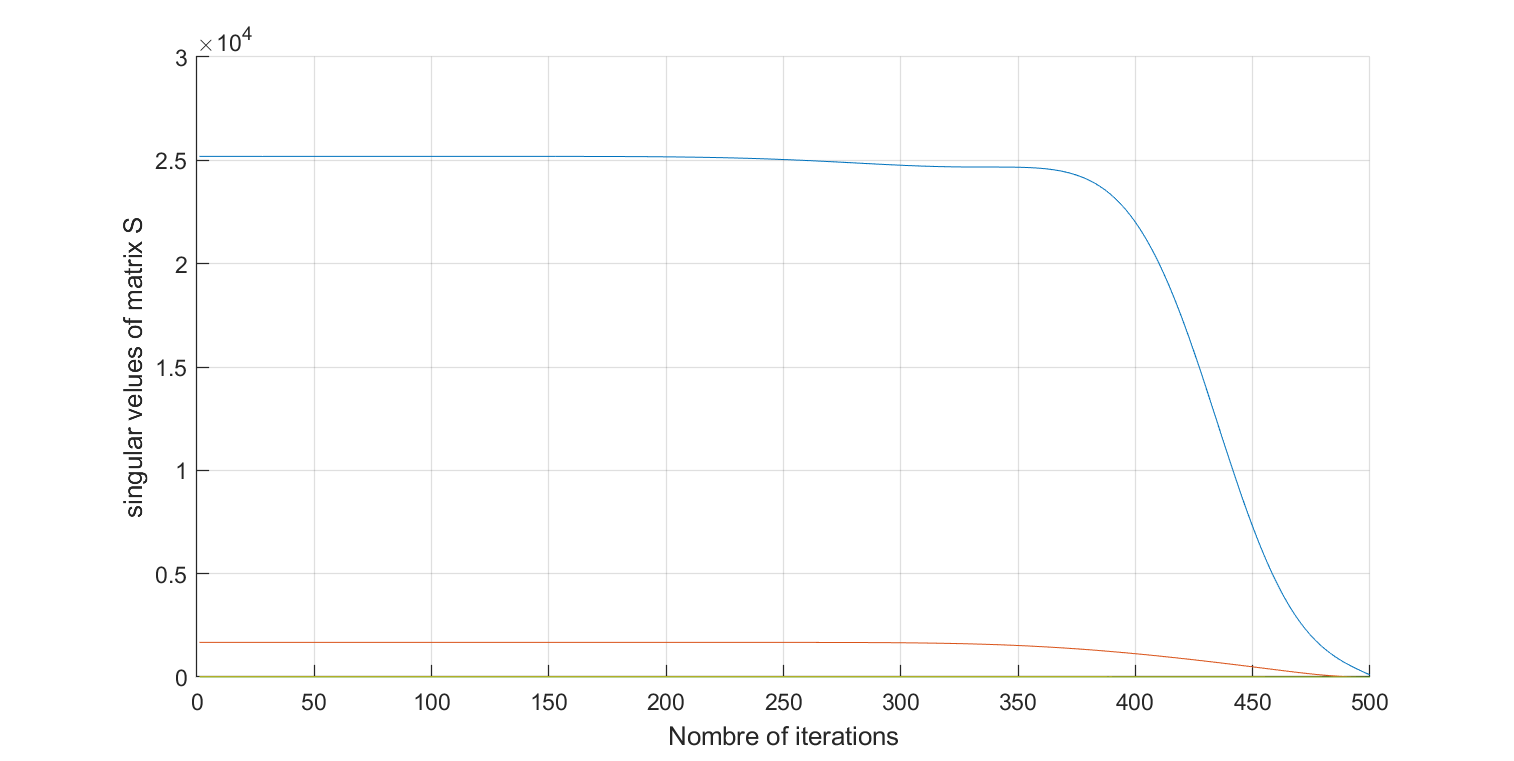
\includegraphics[width = 0.7\linewidth]{Latex report/image/ex2/svds.png}
    \caption{Evolution of singular values of S while solving the Riccati equation}
    \label{fig:svds}
\end{figure}




\subsection{Report the explicit value of the observation close loop poles, and the observer gain resulting
from it.}
The poles of the observer were designed to be 99.9\% of the poles of the closed loop dynamics and the following values have been found (3 significant digits) :

\begin{equation}
    \text{Observer poles :}
    \left[\begin{array}{c}
         0.999\\
         0.987\\
         0.0154\\
         0.985 + 0.0137i\\
         0.985 - 0.0137i\\
    \end{array}
    \right]
\end{equation}

Then by placing the poles of the observer, one may find the following observer gain :

\begin{equation}
    L = 
    \left[ {\begin{array}{ccccc}
        0.9845 &0  &0      &0.01   &0         \\
        0      &50 &0.0299 &0      &0         \\
        0      &0  &0.0083 &0      &0.0008    \\
        0      &0  &0      &0.0032 &0         \\
        0      &0  &0      &0      &-0.0478   \\
    \end{array} } \right] 
\end{equation}

\subsection{Provide a screen shot of your final Simulink scheme and the submodules you had to complete.}
\begin{figure}[H]
    \centering
    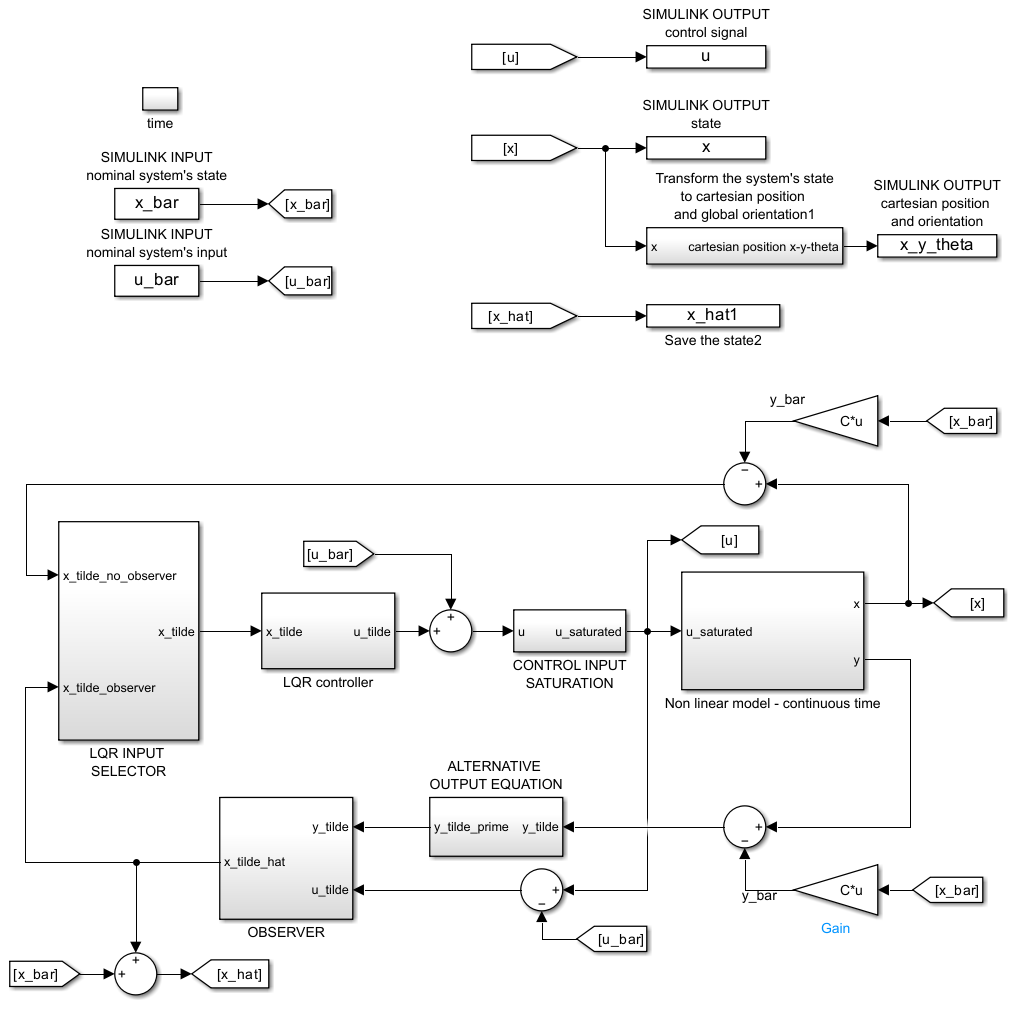
\includegraphics[width = 0.8\linewidth]{Latex report/image/ex2Simulink.png}
    \caption{Simulink diagram of exercise 2}
    \label{fig:ex2Simulink}
\end{figure}


\begin{figure}[H]
    \centering
         \begin{subfigure}[b]{0.8\textwidth}
         \centering
         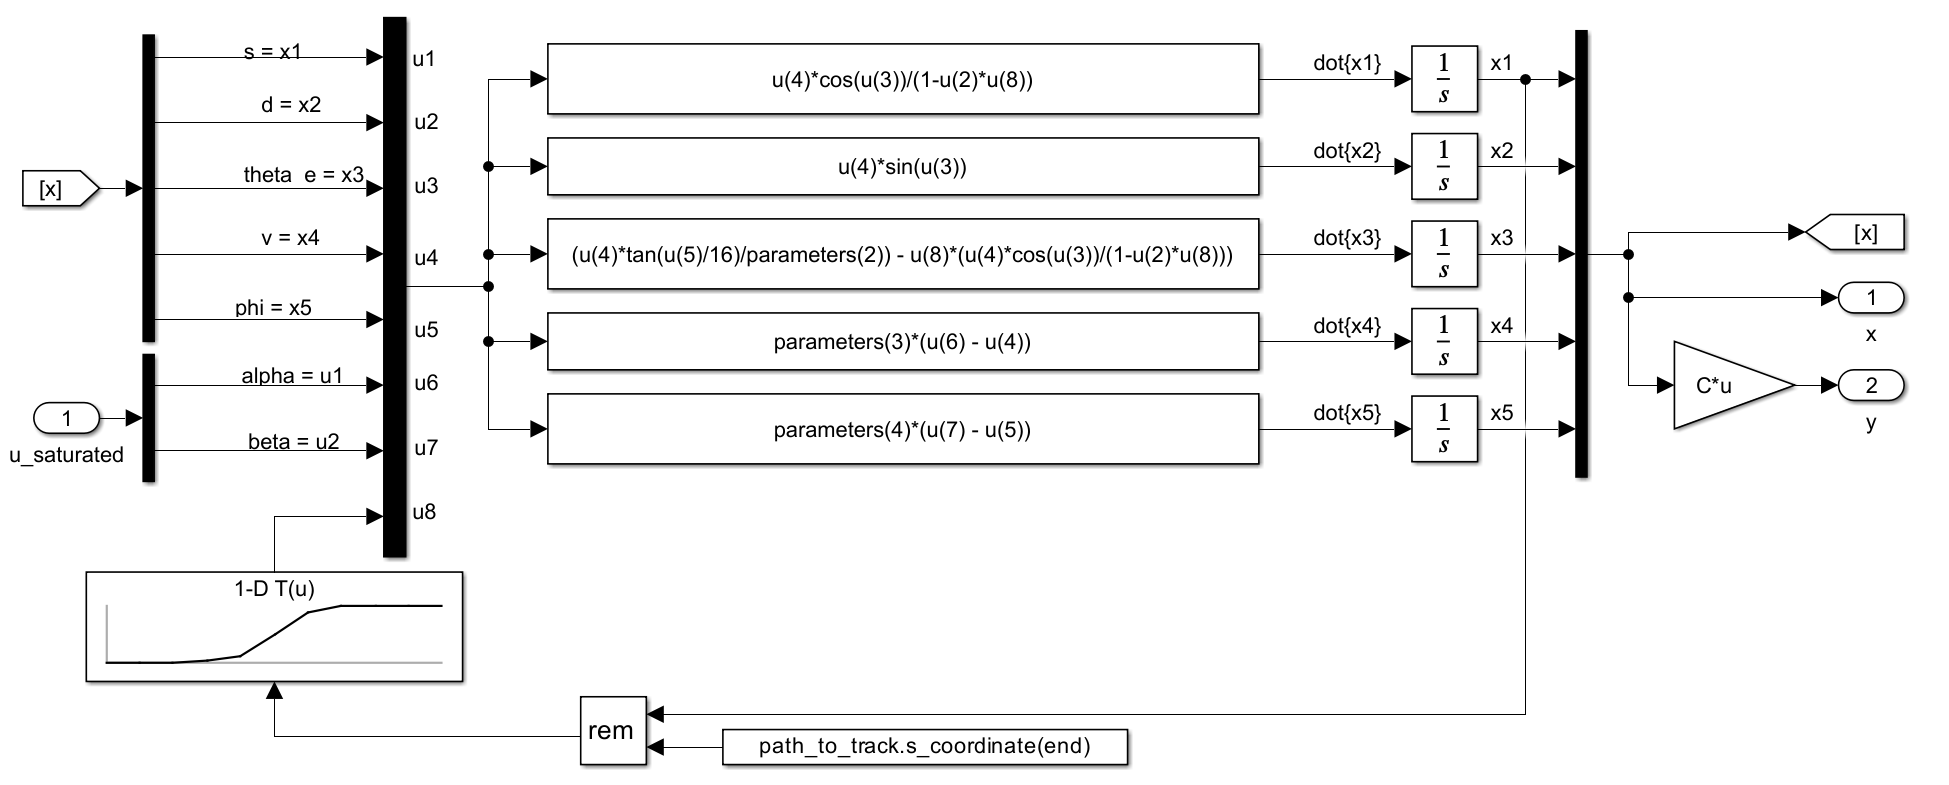
\includegraphics[width=\textwidth]{Latex report/image/nonLinModelContinousTimeEx2.png}
         \caption{Non linear model in continuous time implementation}
         \label{fig:nonLinSimulinkex2}
     \end{subfigure}
     \begin{subfigure}[b]{0.45\textwidth}
         \centering
         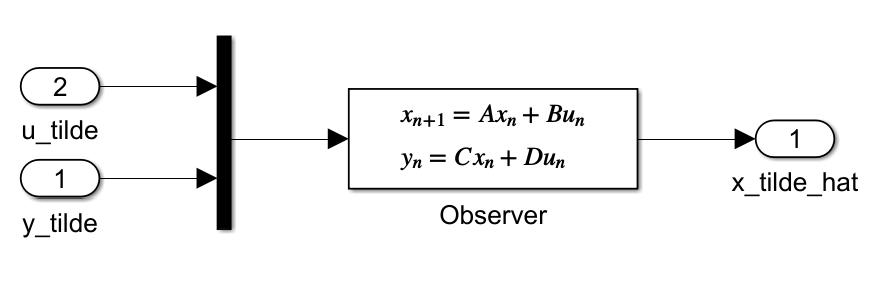
\includegraphics[width=\textwidth]{Latex report/image/ex2Observer.png}
         \caption{Observer implementation}
         \label{fig:ObsSim}
     \end{subfigure}
     \begin{subfigure}[b]{0.45\textwidth}
         \centering
         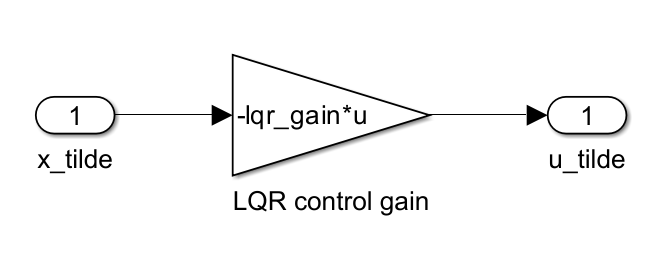
\includegraphics[width=\textwidth]{Latex report/image/Ex2LQR.png}
         \caption{LQR implementation}
         \label{fig:lqrSim}
     \end{subfigure}
     \begin{subfigure}[b]{0.45\textwidth}
         \centering
         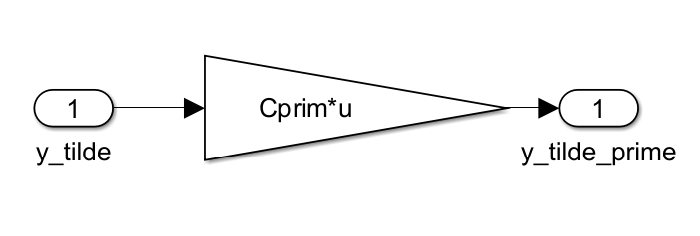
\includegraphics[width=\textwidth]{Latex report/image/ex2altEq.png}
         \caption{Alternative equation implementation}
         \label{fig:altEqSim}
     \end{subfigure}
     \begin{subfigure}[b]{0.45\textwidth}
         \centering
         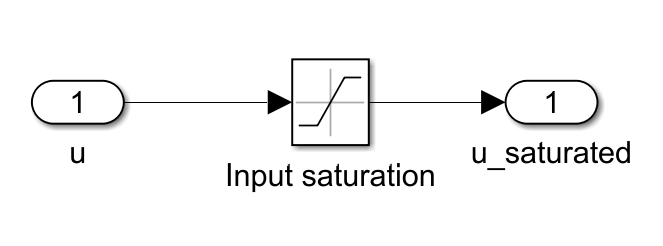
\includegraphics[width=\textwidth]{Latex report/image/ex2Saturation.png}
         \caption{Input saturation implementation}
         \label{fig:simSat}
     \end{subfigure}
    \caption{Implementation of the required block in simulink for exercise 2}
    \label{fig:simImplEx2}
\end{figure}

\subsection{Report the simulation results for the proposed values.}

\begin{figure}[H]
    \centering
     \begin{subfigure}[b]{0.45\textwidth}
         \centering
         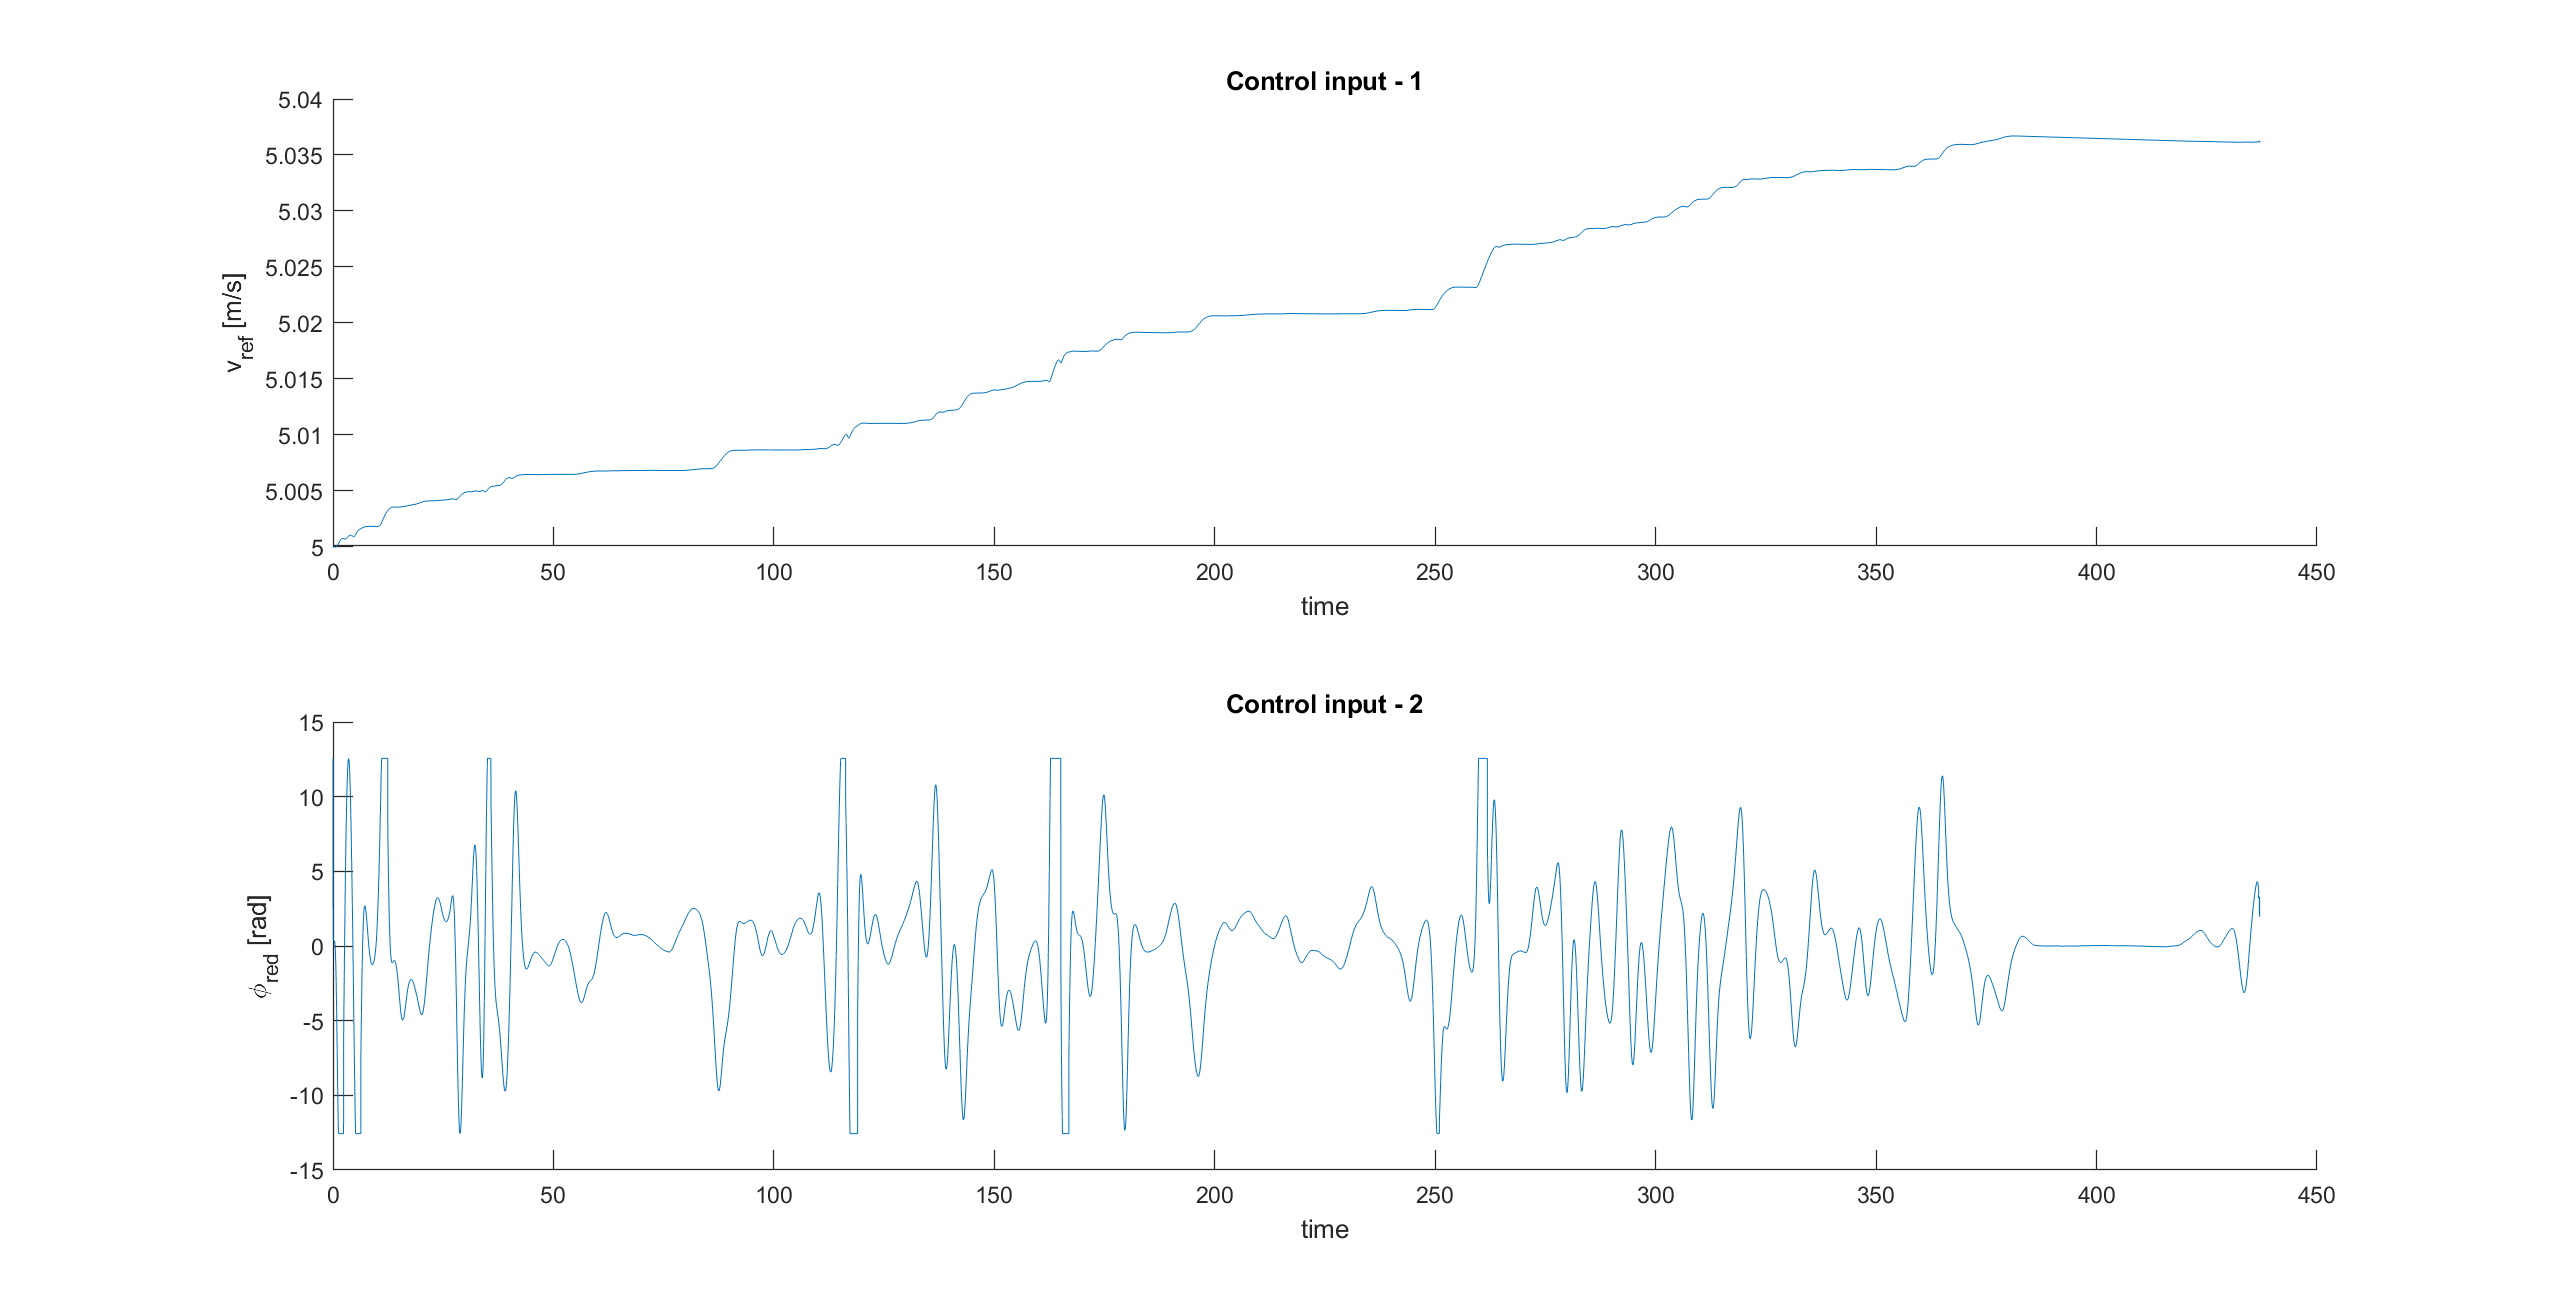
\includegraphics[width=\textwidth]{Latex report/image/ex2/input.png}
         \caption{Control input}
         \label{fig:input}
     \end{subfigure}
     \begin{subfigure}[b]{0.45\textwidth}
         \centering
         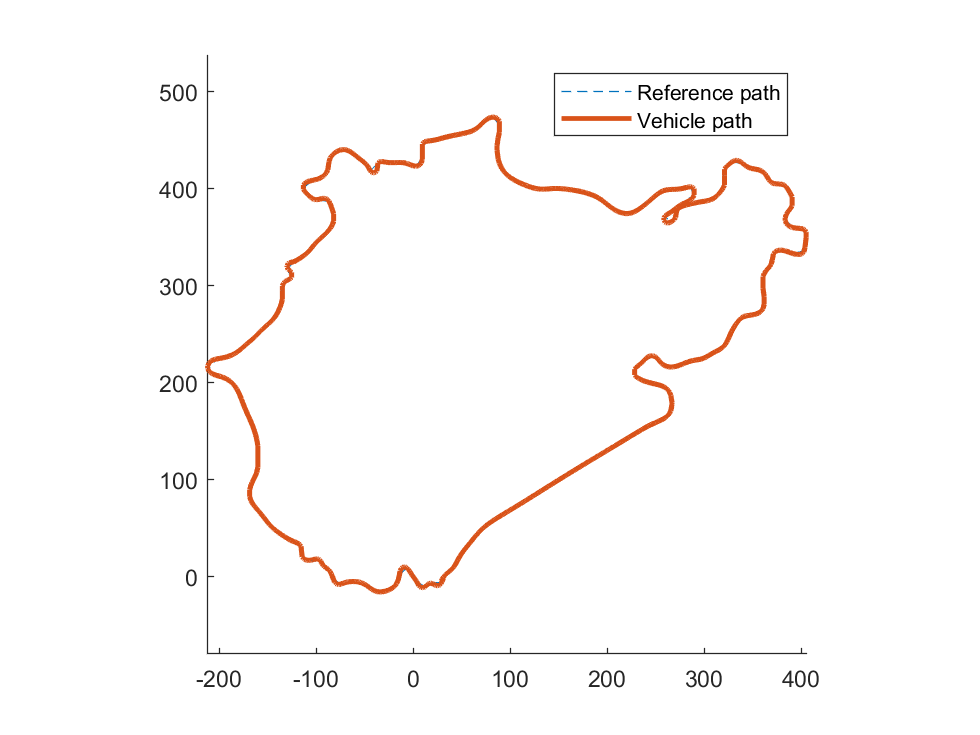
\includegraphics[width=\textwidth]{Latex report/image/ex2/trajectory.png}
         \caption{Trajectory}
         \label{fig:traj}
     \end{subfigure}
     \begin{subfigure}[b]{0.8\textwidth}
         \centering
         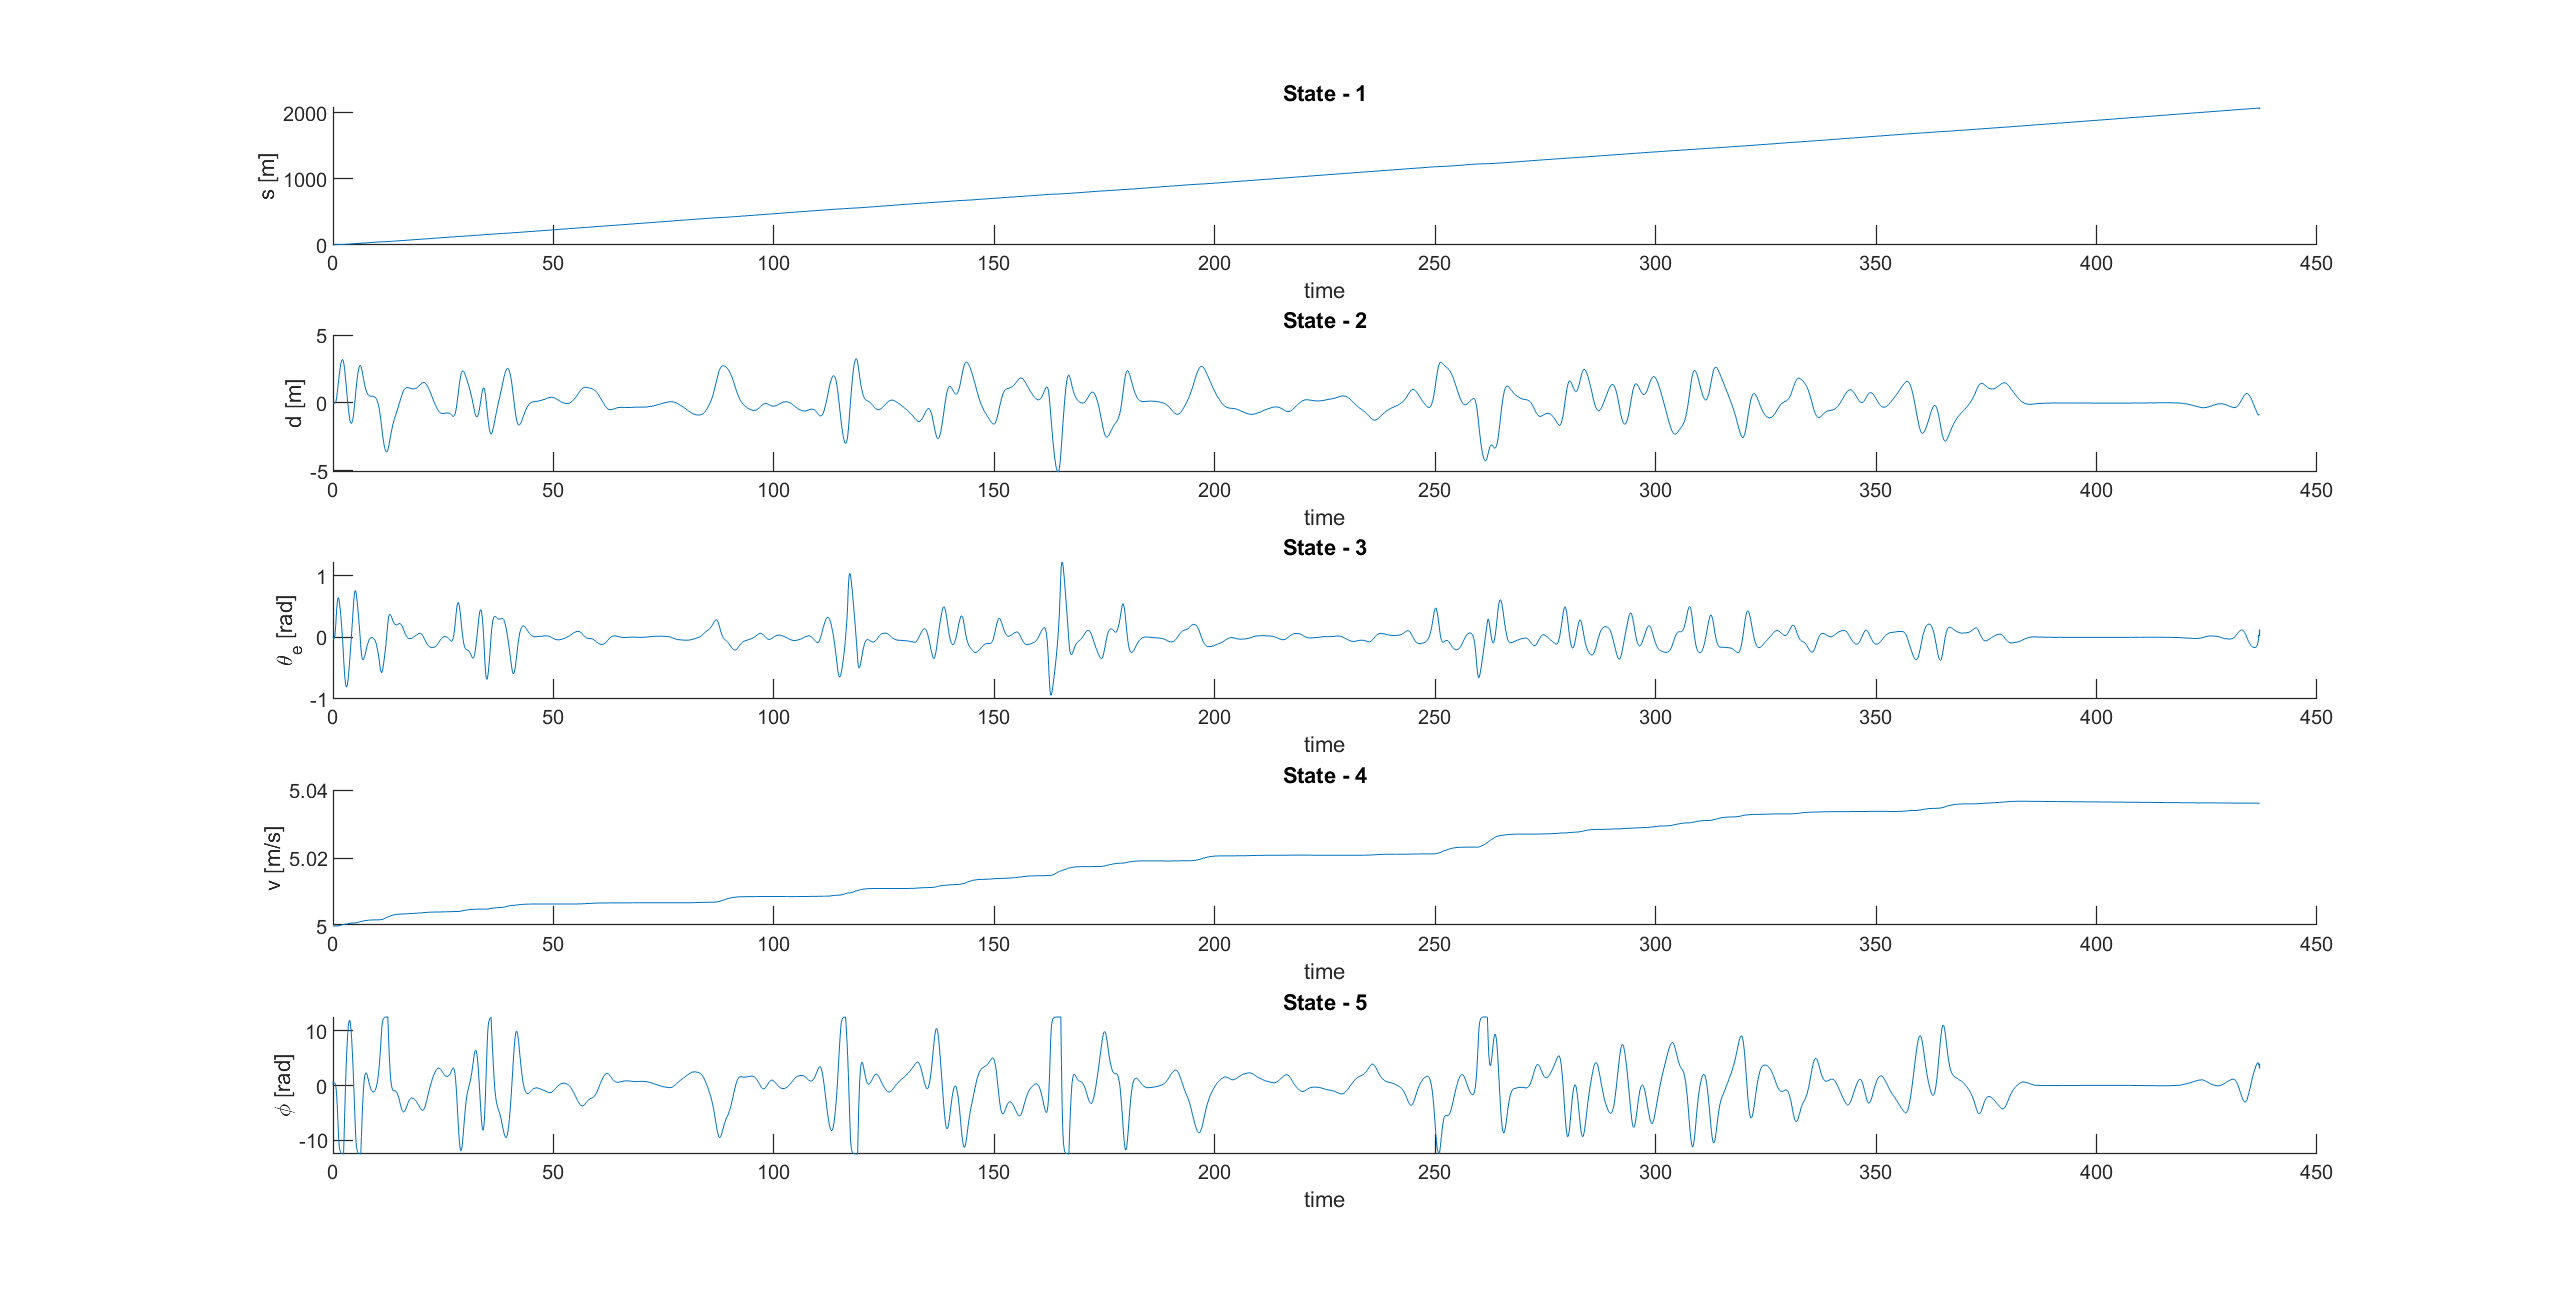
\includegraphics[width=\textwidth]{Latex report/image/ex2/state.png}
         \caption{Observed state}
         \label{fig:State}
     \end{subfigure}
     \begin{subfigure}[b]{0.8\textwidth}
         \centering
         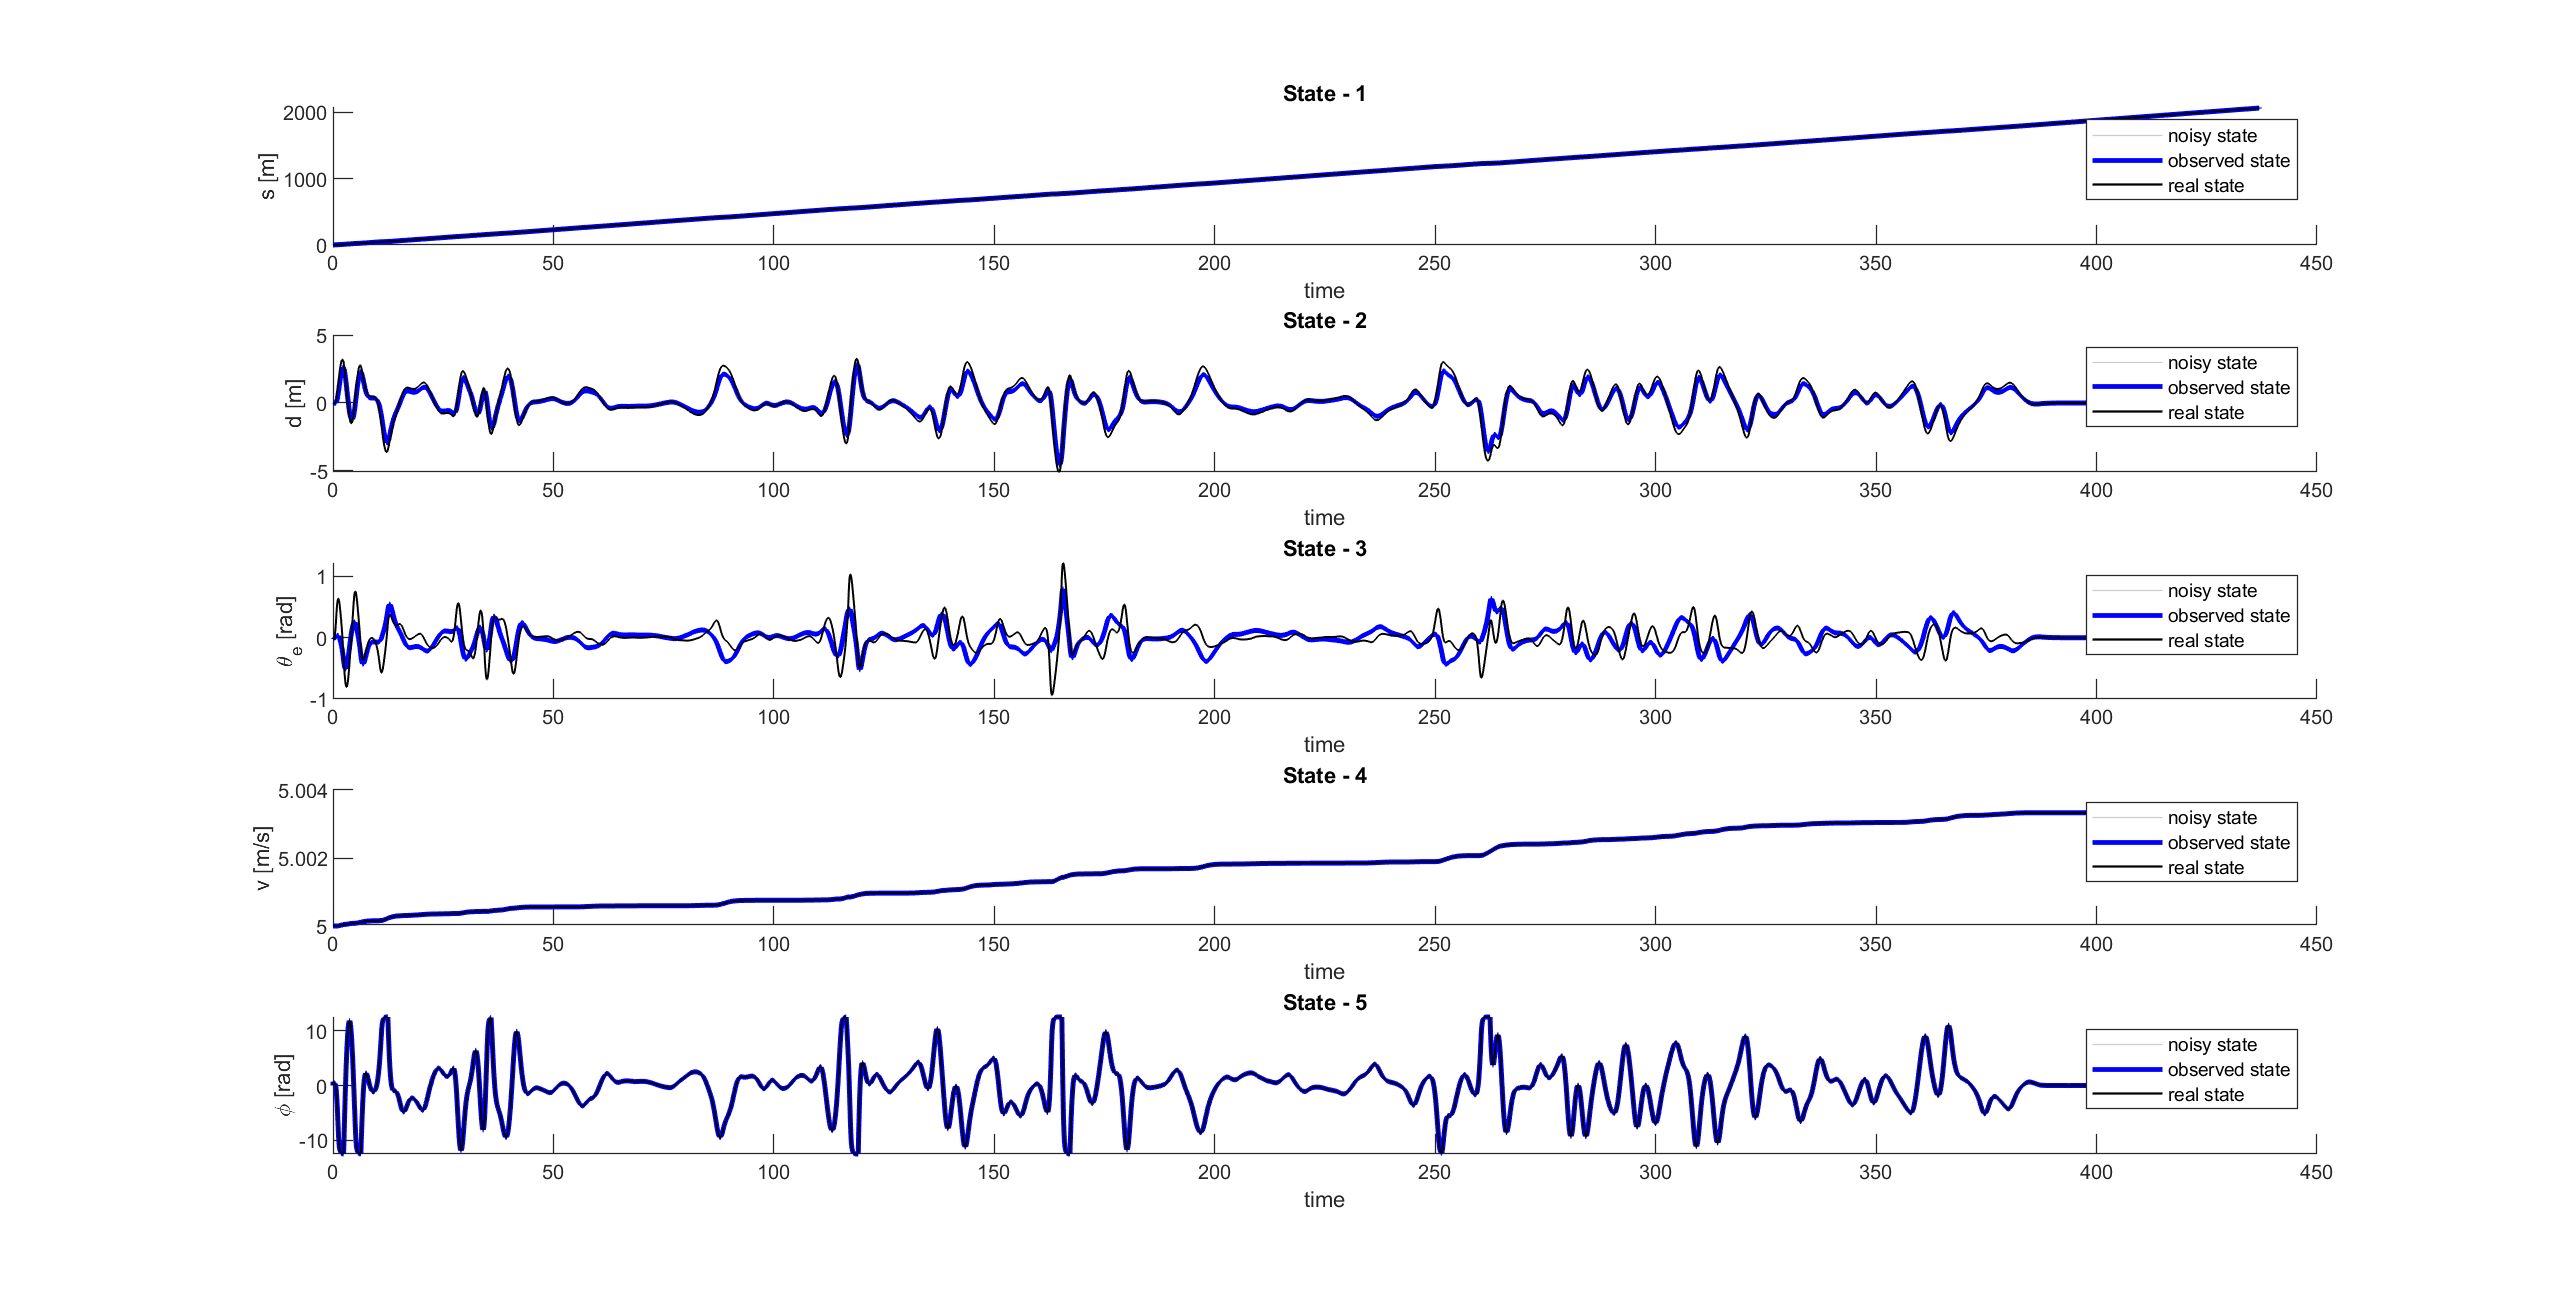
\includegraphics[width=\textwidth]{Latex report/image/ex2/obs.png}
         \caption{Comparison with state measurement}
         \label{fig:Obs}
     \end{subfigure}
    \caption{Simulation of the LQR regulator with an observer and new pole placement}
    \label{fig:sim}
\end{figure}

\subsection{The proposed value of Q1 intends to assign very little importance to the error deriving from x1. Could you explain why doing this might make sense?}
First of all, $x_1$ represents $s$, the distance travelled along the path, which is a function of all the other variables (indirectly for $x_5$), whereas none of the other variables is a function of $x_1$. Therefore, all corrections to the other variables correct $x_1$, whereas corrections to $x_1$ do not correct the other variables. For example, correcting $x_2$ or $x_3$, which represent tracking errors, allows $X_1$ to be controlled efficiently. Indeed, if $x_2$ and $x_3$ are zero, then we are sure to be on the path.
On the other hand, if we give great importance to the control of $x_1$, we would inevitably induce more error in the other variables, which as we have seen, induce error in $x_1$, which would be counterproductive. Therefore it make completly sense to assign very little weight to the control of $x_1$



\subsection{Propose a different pair Q1 and Q2 such that heading deviation error is highly penalized compared to the other states and report simulation results where the impact of doing so can be clearly observed.}
The new proposed $Q_1$ and $Q_2$ are :
\begin{equation}
    Q_1 = 
    \left[ {\begin{array}{ccccc}
        1e-5 &0   &0   &0   &0     \\
        0    &0.5 &0   &0   &0     \\
        0    &0   &50  &0   &0     \\
        0    &0   &0   &0.5 &0     \\
        0    &0   &0   &0   &0.5   \\
    \end{array} } \right]    
    ,\quad
    Q_2 =
    \left[ {\begin{array}{cc}
        1 &0\\
        0 &2e-5\\
    \end{array} } \right]
\end{equation}

The value of the LQR gain obtained by solving the Riccati equation are :
\begin{equation}
    K_{LQR} = 
    \left[ {\begin{array}{ccccc}
         3.99e-4 &0       &0       &0.2237 &0      \\
         0         &20.067 &304.03 &0      &19.308 \\
    \end{array}}\right]
\end{equation}

\begin{figure}[H]
    \centering
     \begin{subfigure}[b]{0.45\textwidth}
         \centering
         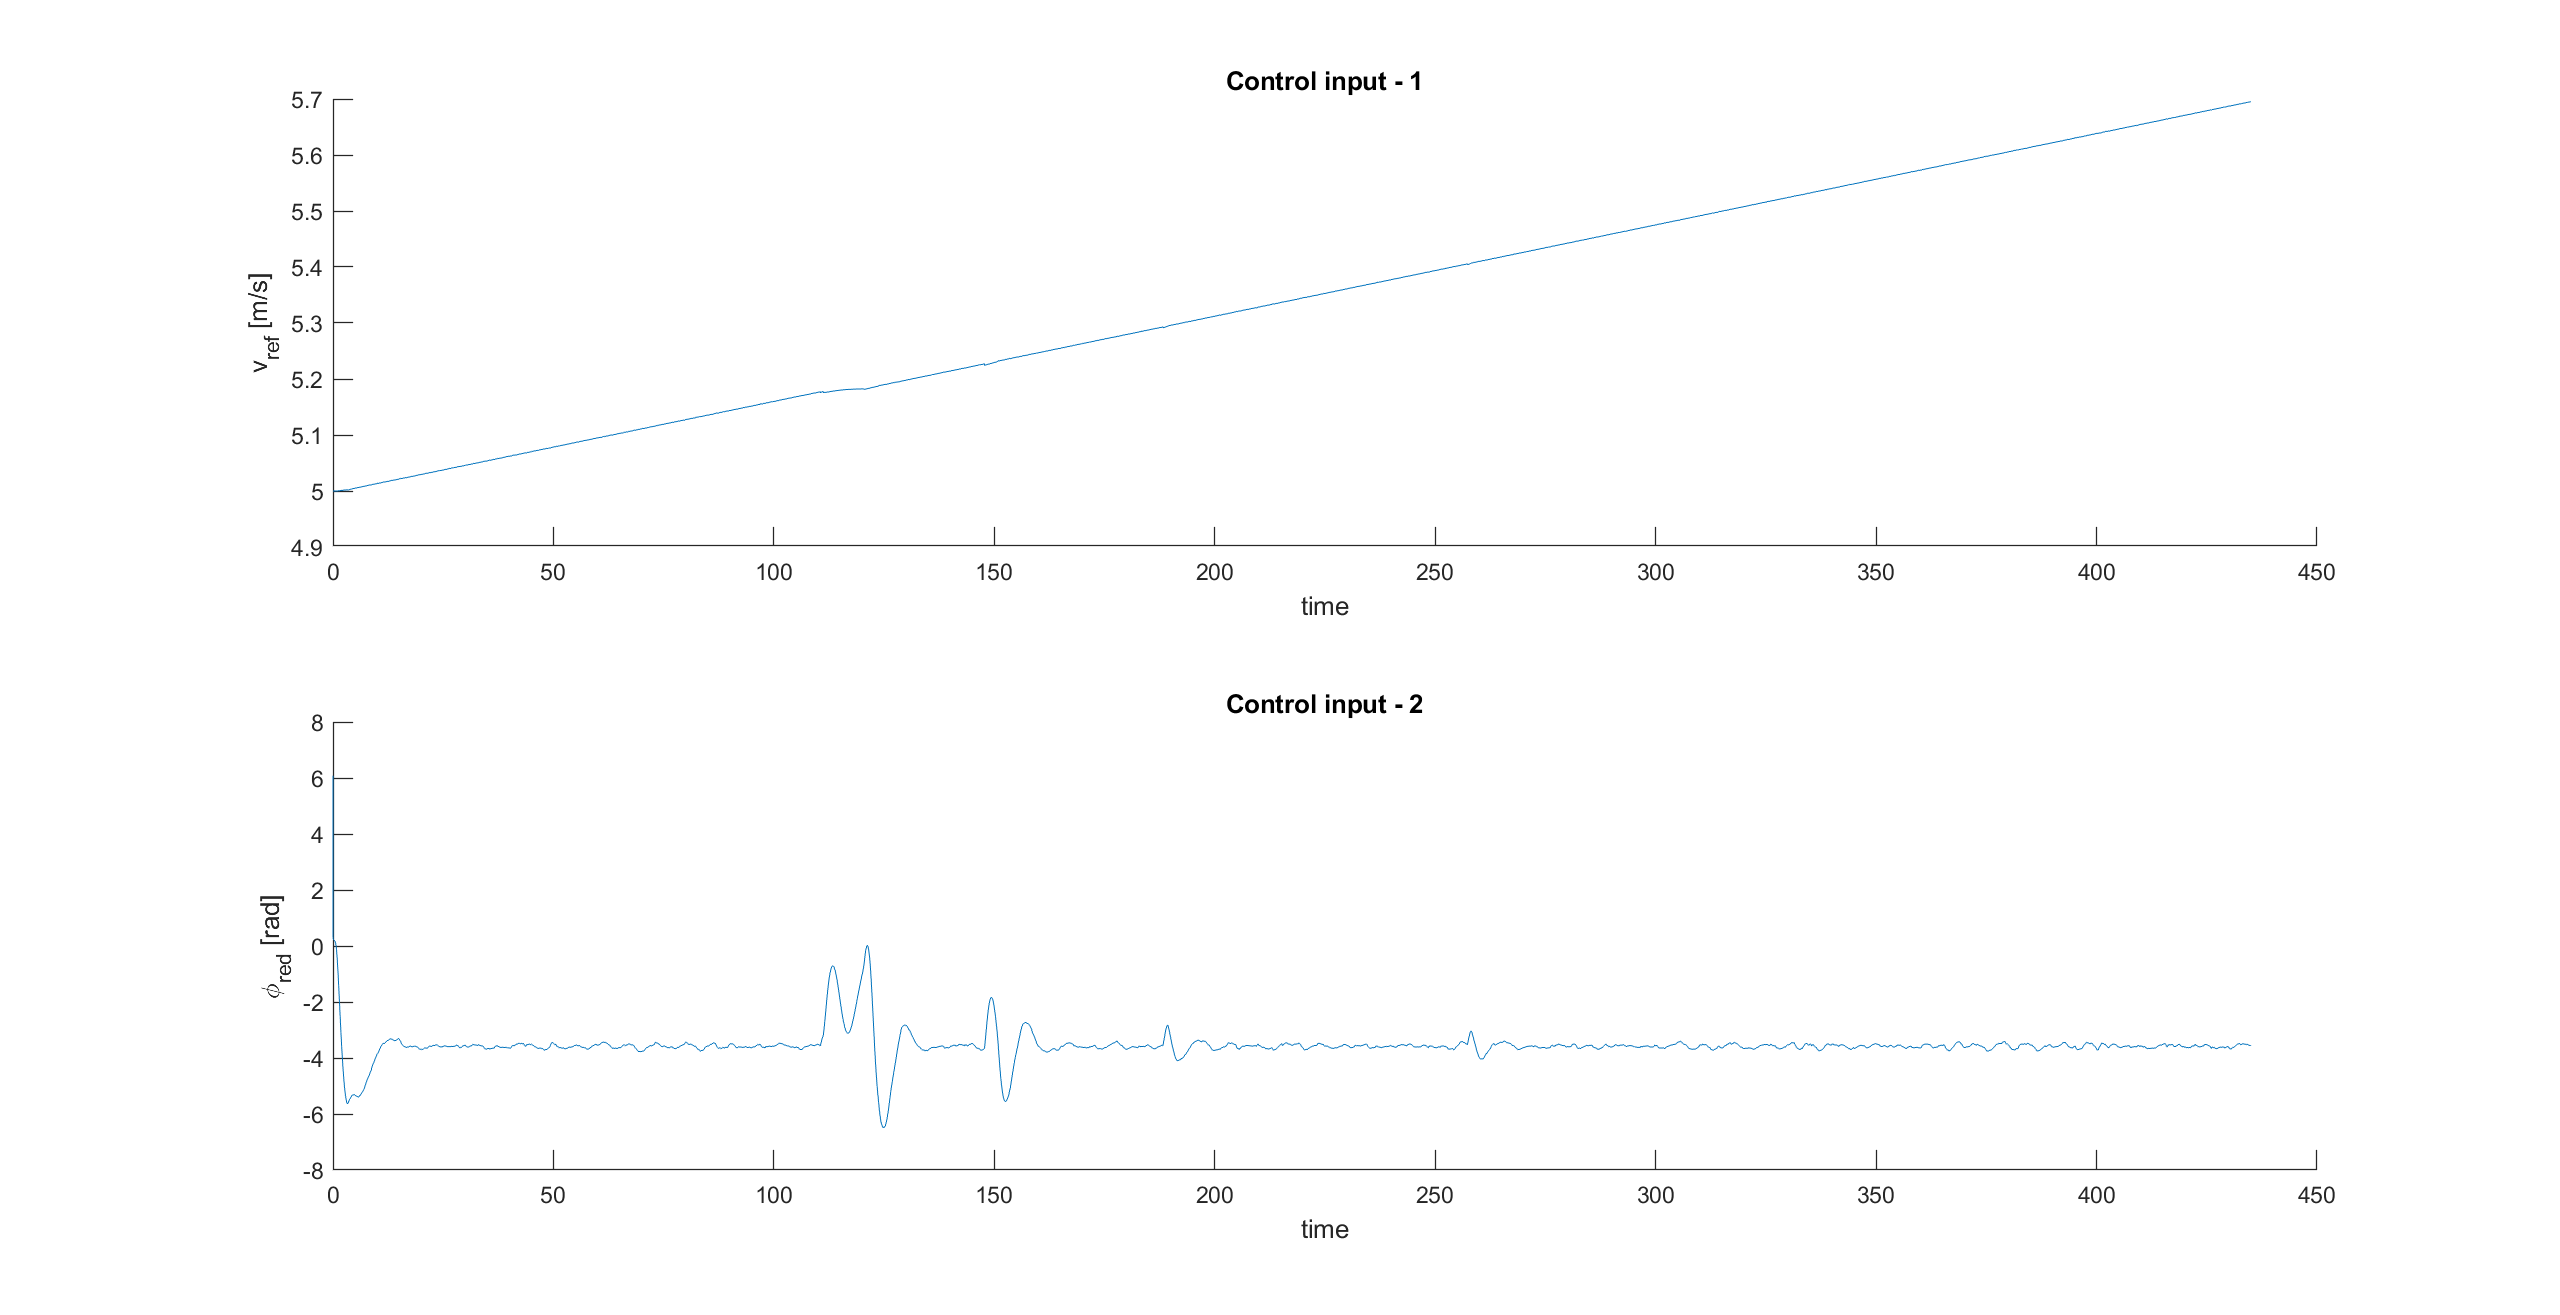
\includegraphics[width=\textwidth]{Latex report/image/ex2/input2.png}
         \caption{Control input}
         \label{fig:2input}
     \end{subfigure}
     \begin{subfigure}[b]{0.45\textwidth}
         \centering
         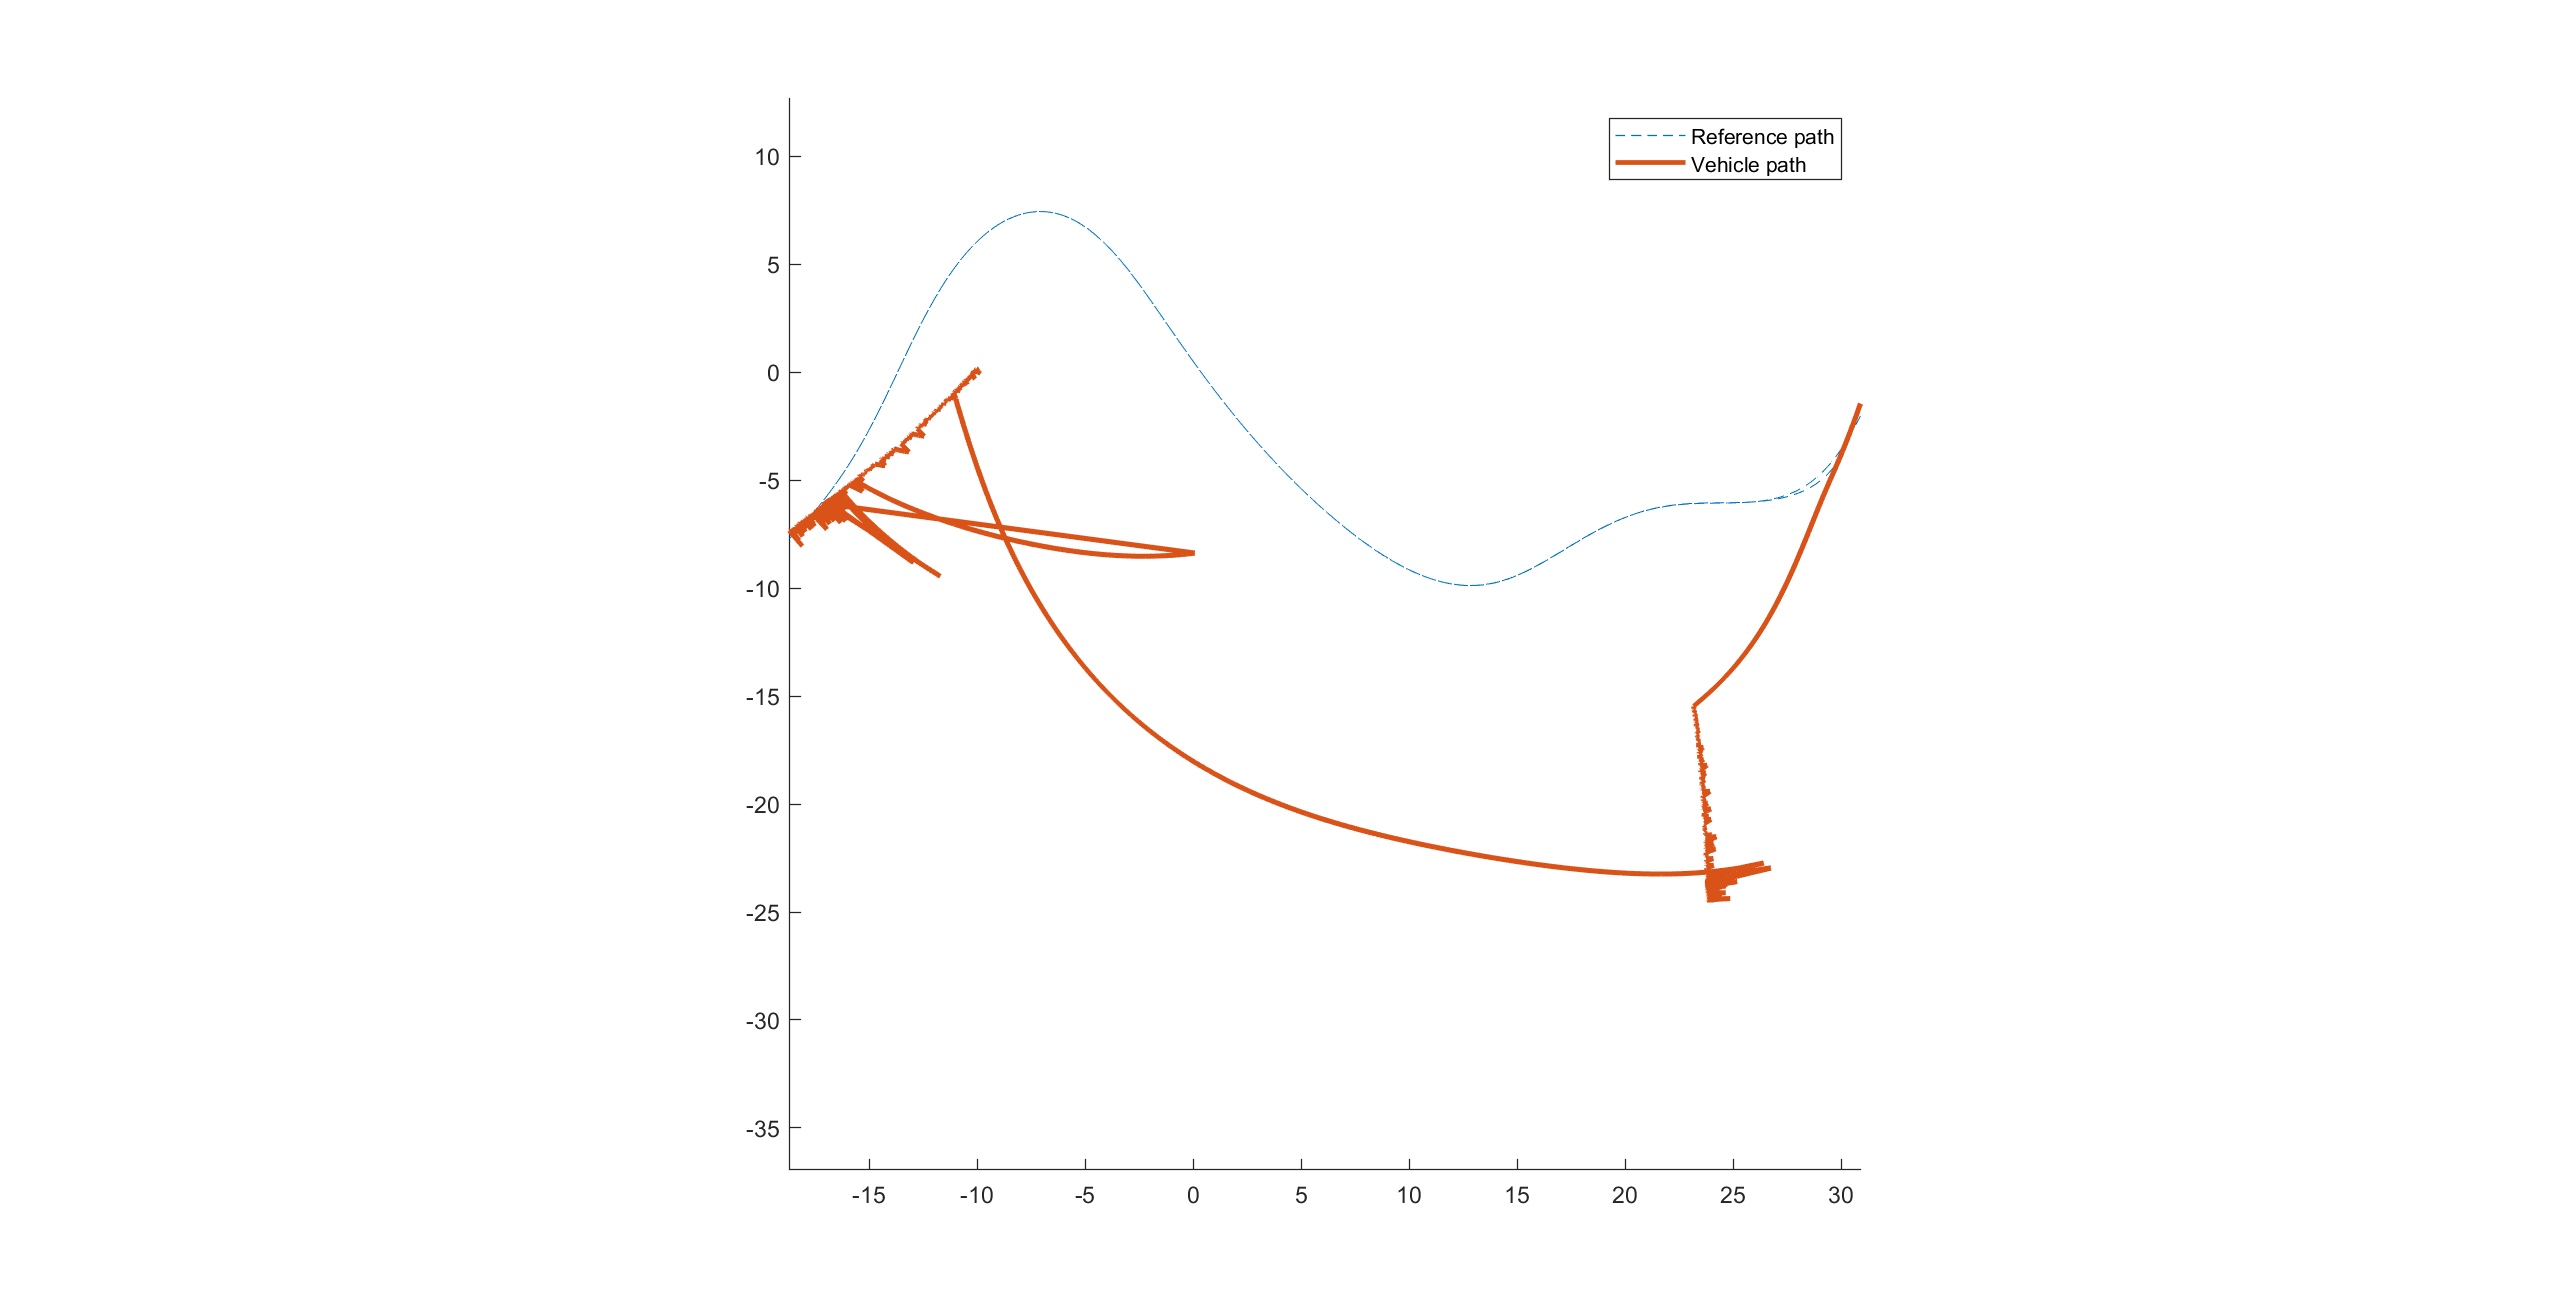
\includegraphics[width=\textwidth]{Latex report/image/ex2/trajectory2.png}
         \caption{Trajectory}
         \label{fig:2traj}
     \end{subfigure}
     \begin{subfigure}[b]{0.8\textwidth}
         \centering
         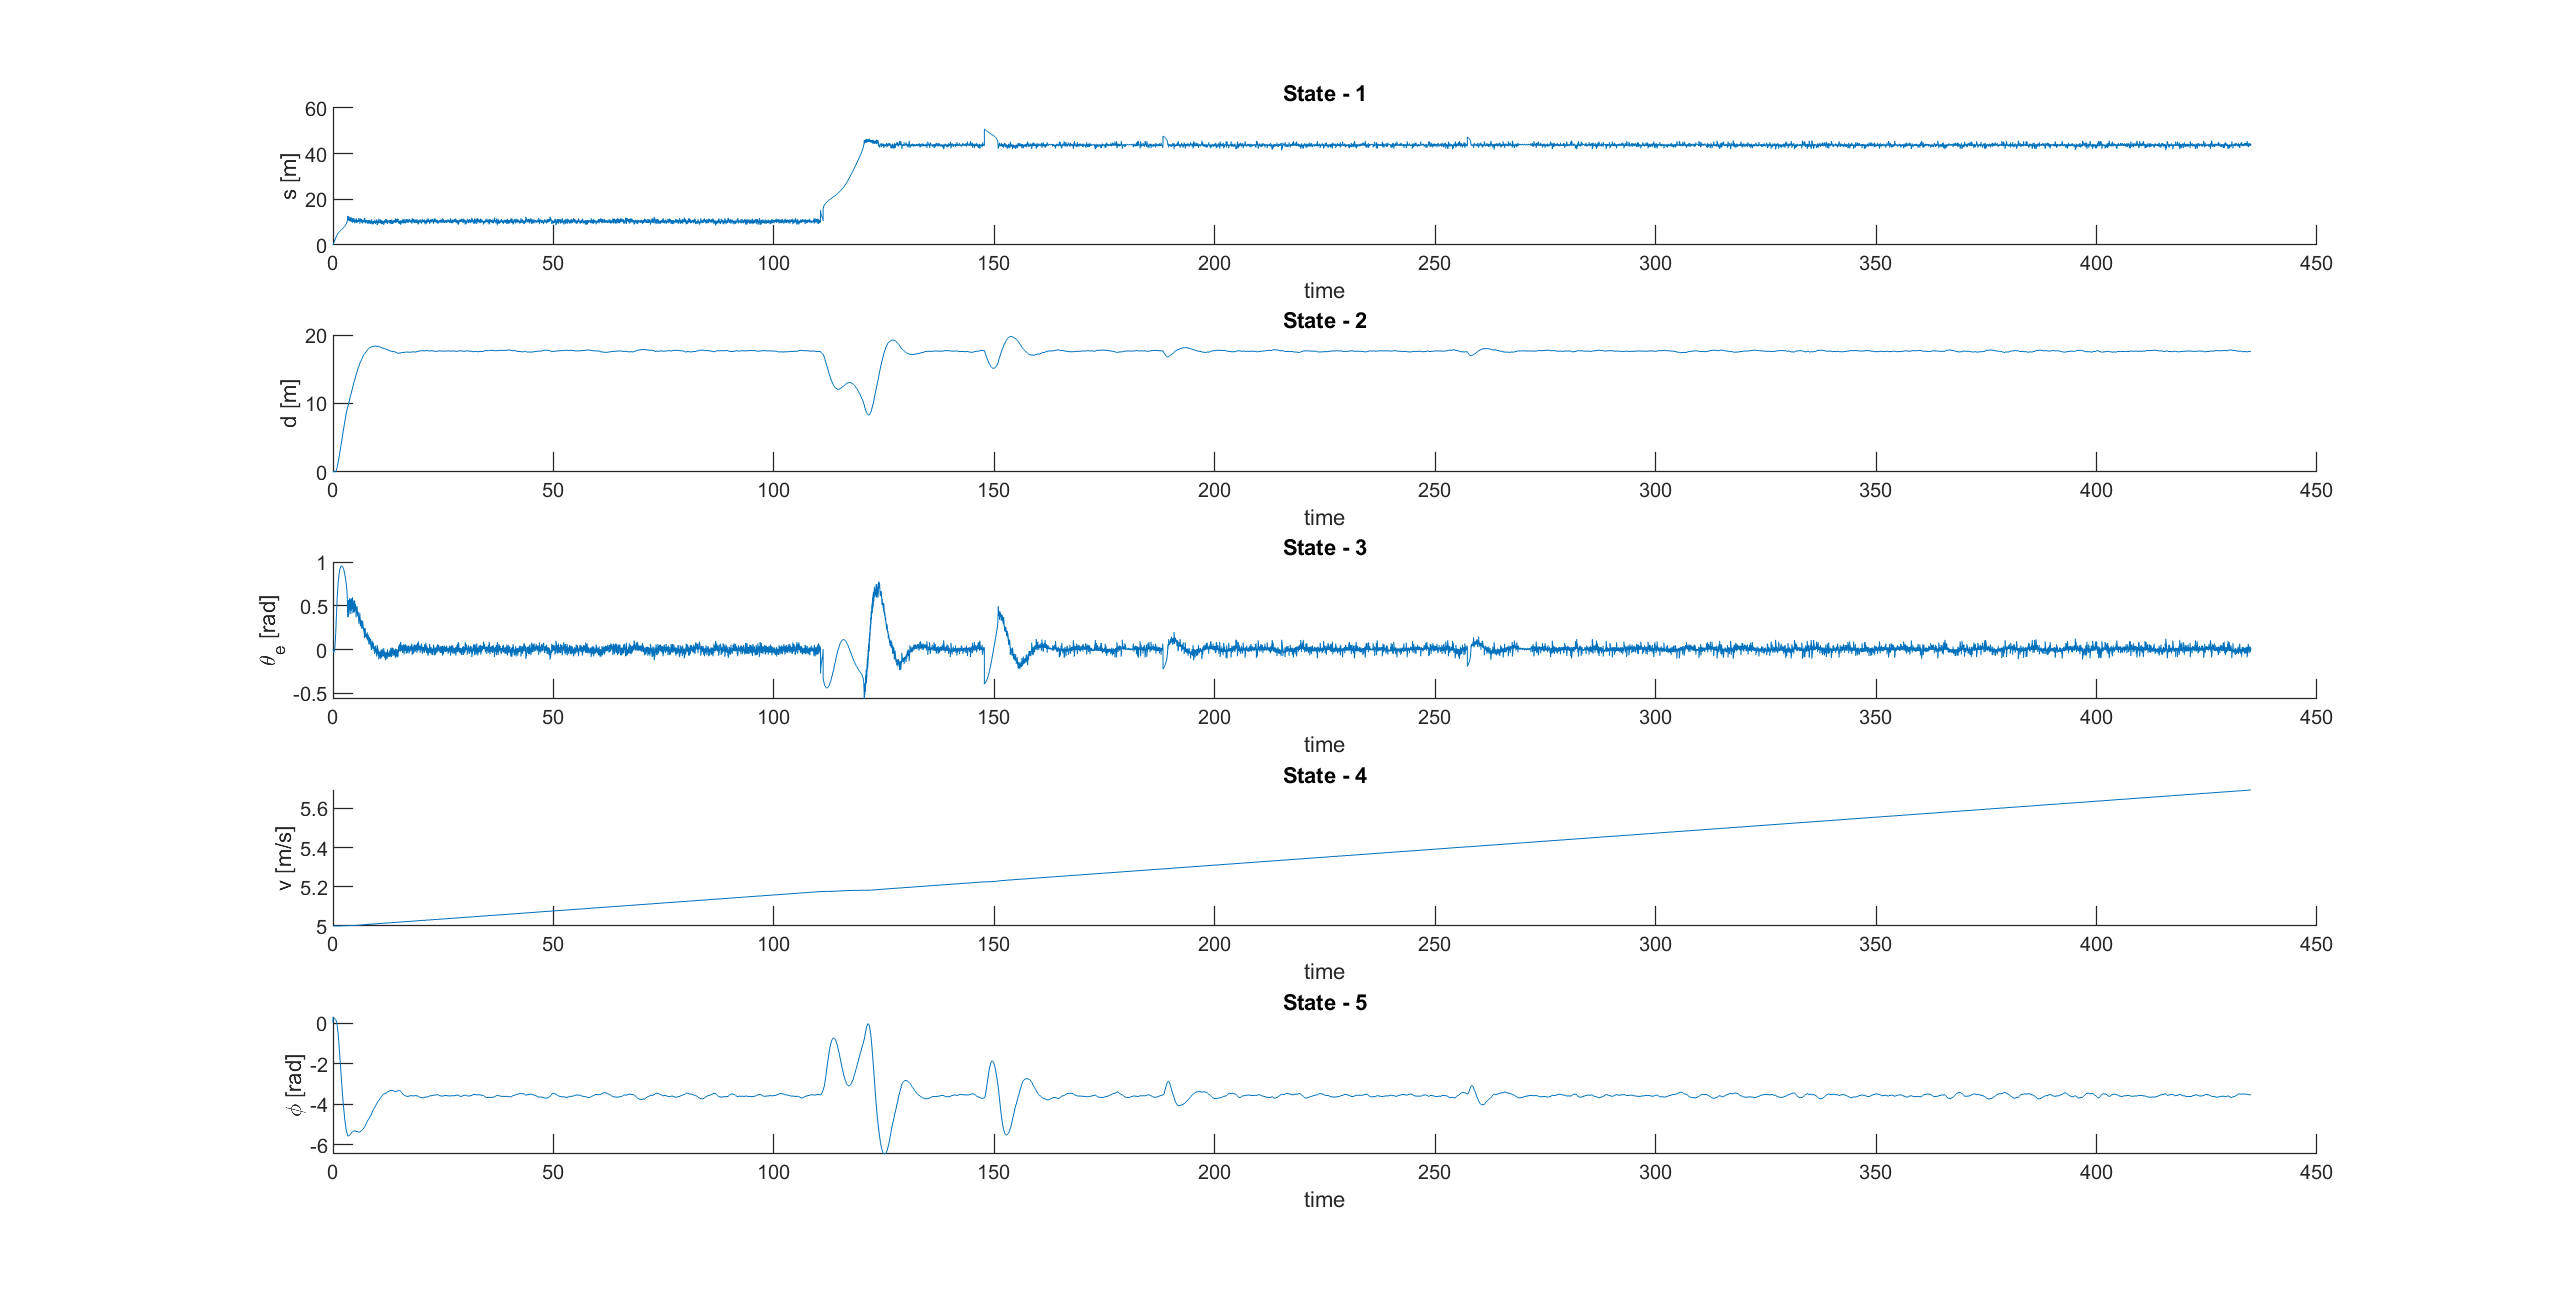
\includegraphics[width=\textwidth]{Latex report/image/ex2/state2.png}
         \caption{Observed state}
         \label{fig:2State}
     \end{subfigure}
     \begin{subfigure}[b]{0.8\textwidth}
         \centering
         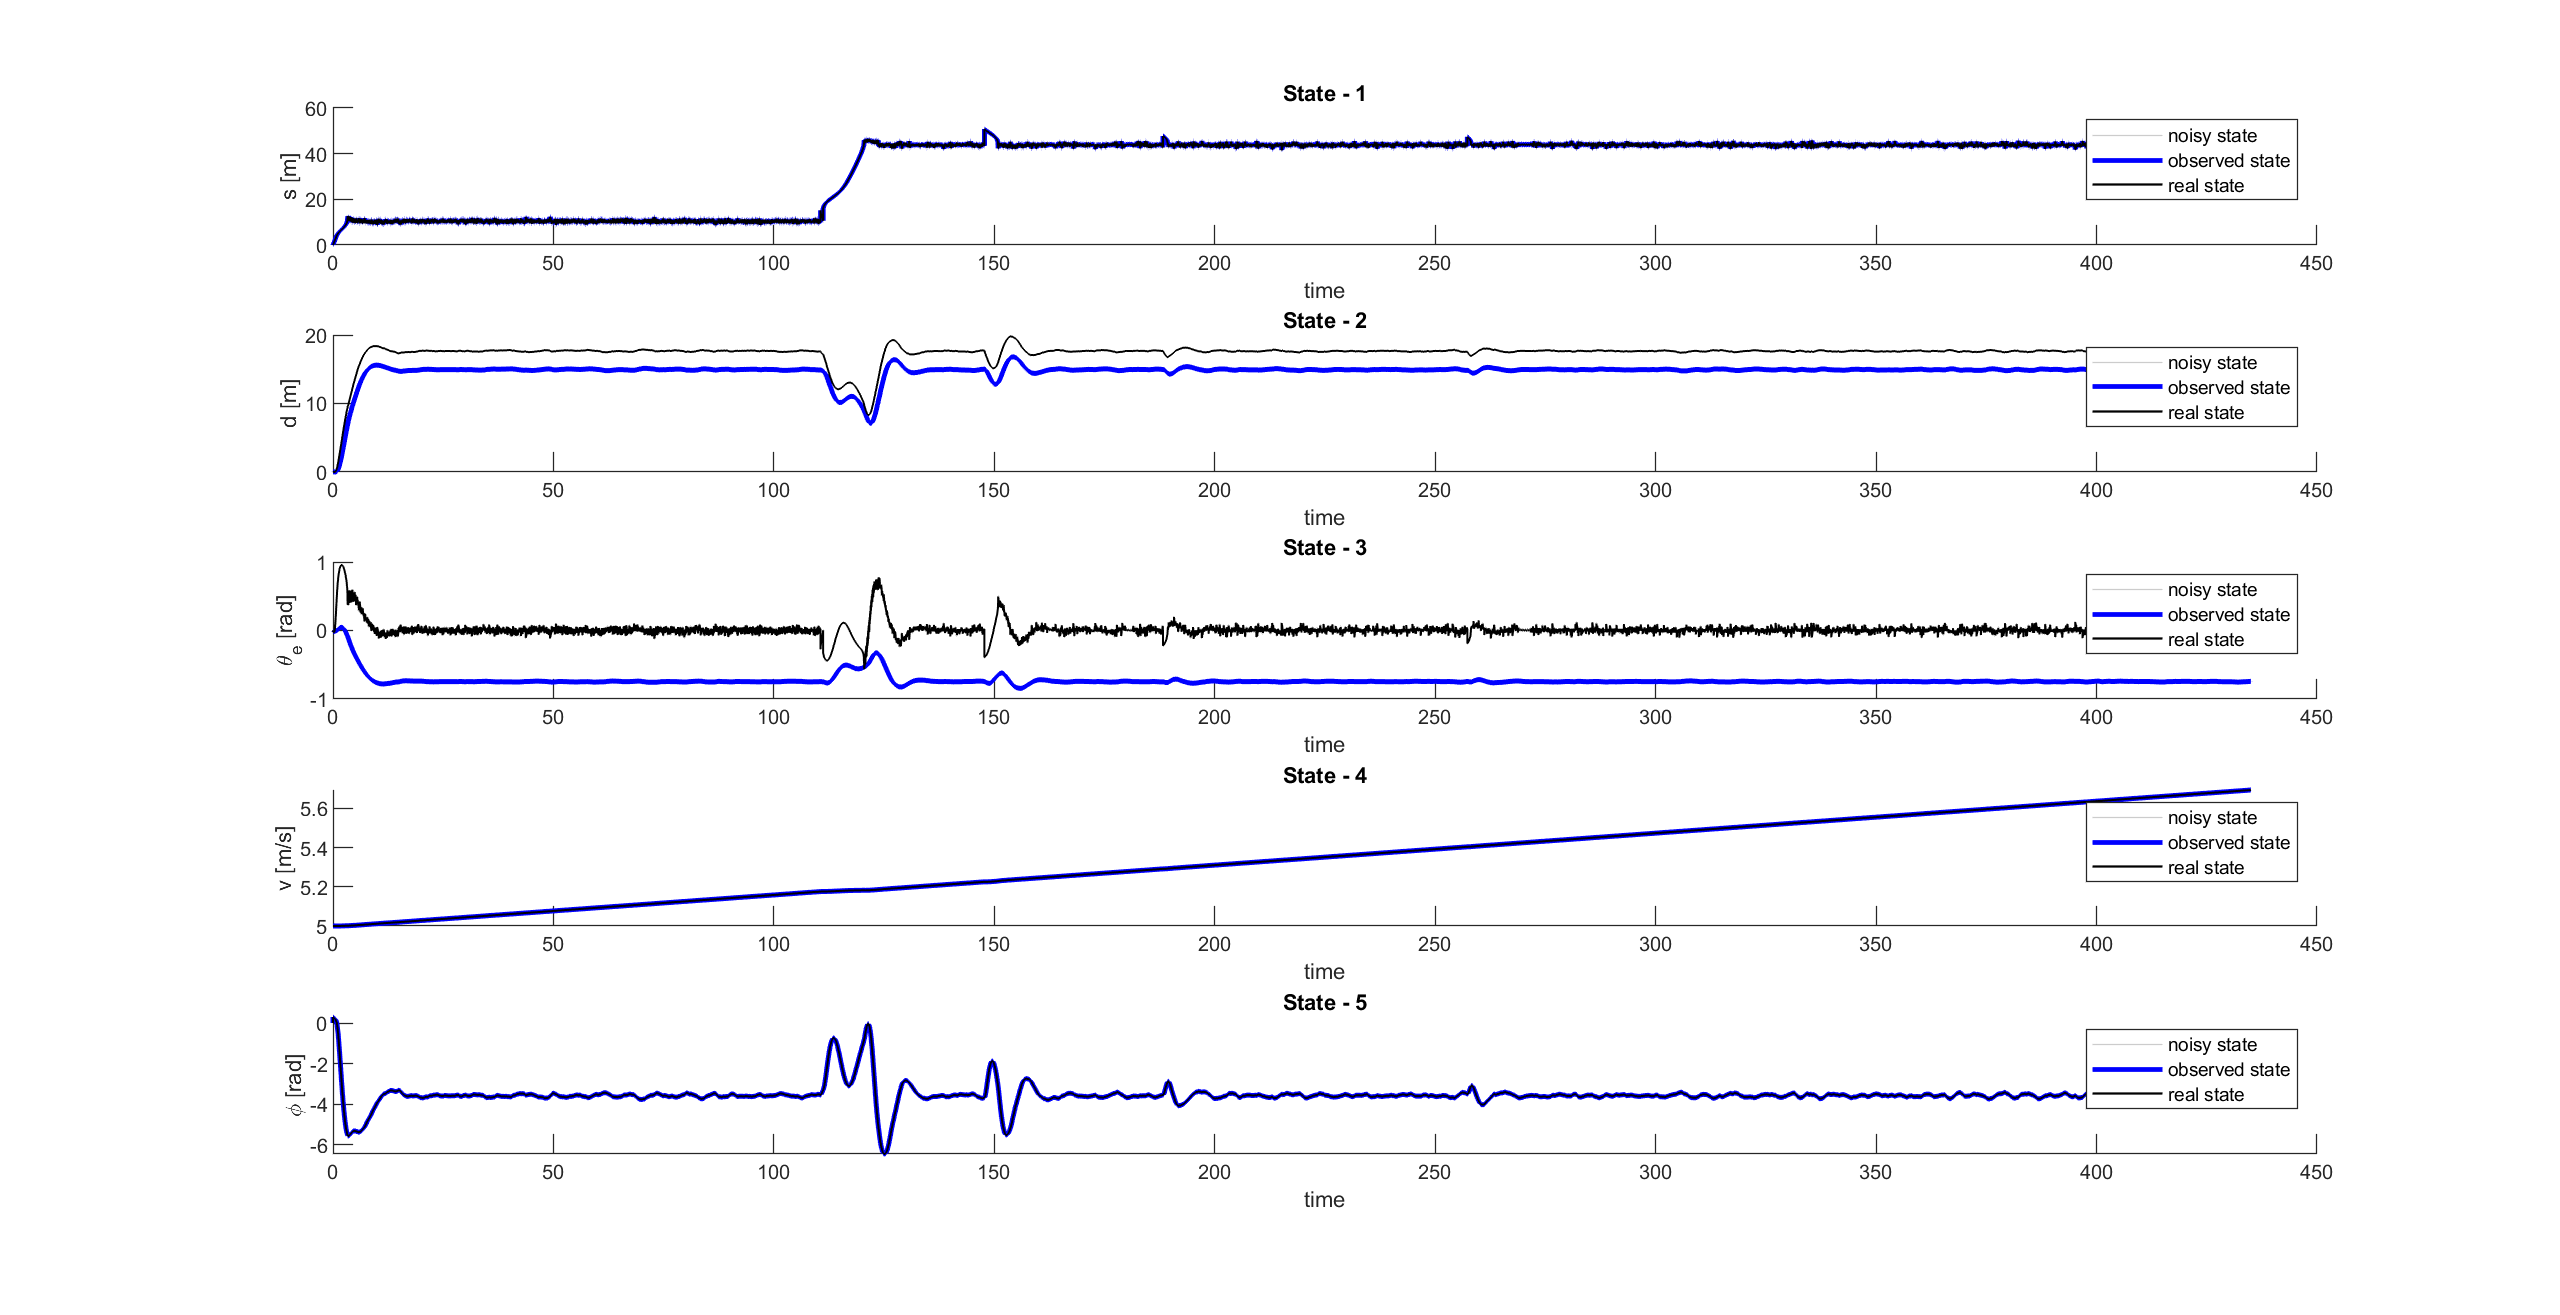
\includegraphics[width=\textwidth]{Latex report/image/ex2/obs2.png}
         \caption{Comparison with state measurement}
         \label{fig:2Obs}
     \end{subfigure}
    \caption{Simulation of the LQR regulator with an observer and new pole placement}
    \label{fig:sim2}
\end{figure}




\subsection{Is the proposed placement for the observation close loop poles appropriate? why? If not,propose a new set of poles to improve the observation performance.}

\begin{figure}[H]
    \centering
     \begin{subfigure}[b]{0.45\textwidth}
         \centering
         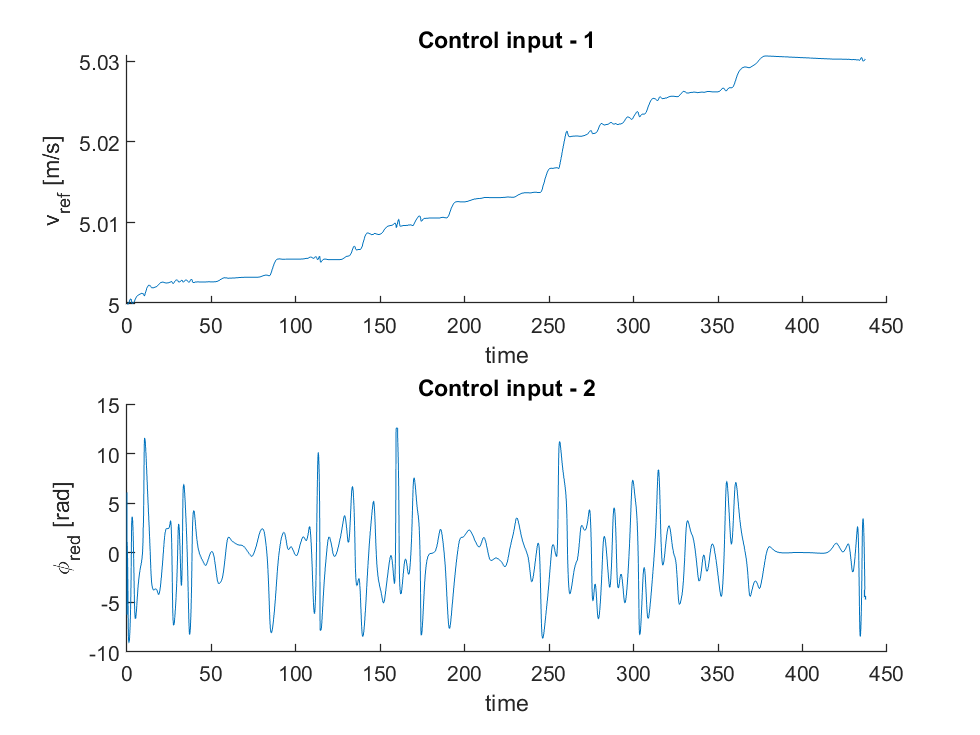
\includegraphics[width=\textwidth]{Latex report/image/ex2/inputNewpole.png}
         \caption{Control input}
         \label{fig:NPinput}
     \end{subfigure}
     \begin{subfigure}[b]{0.45\textwidth}
         \centering
         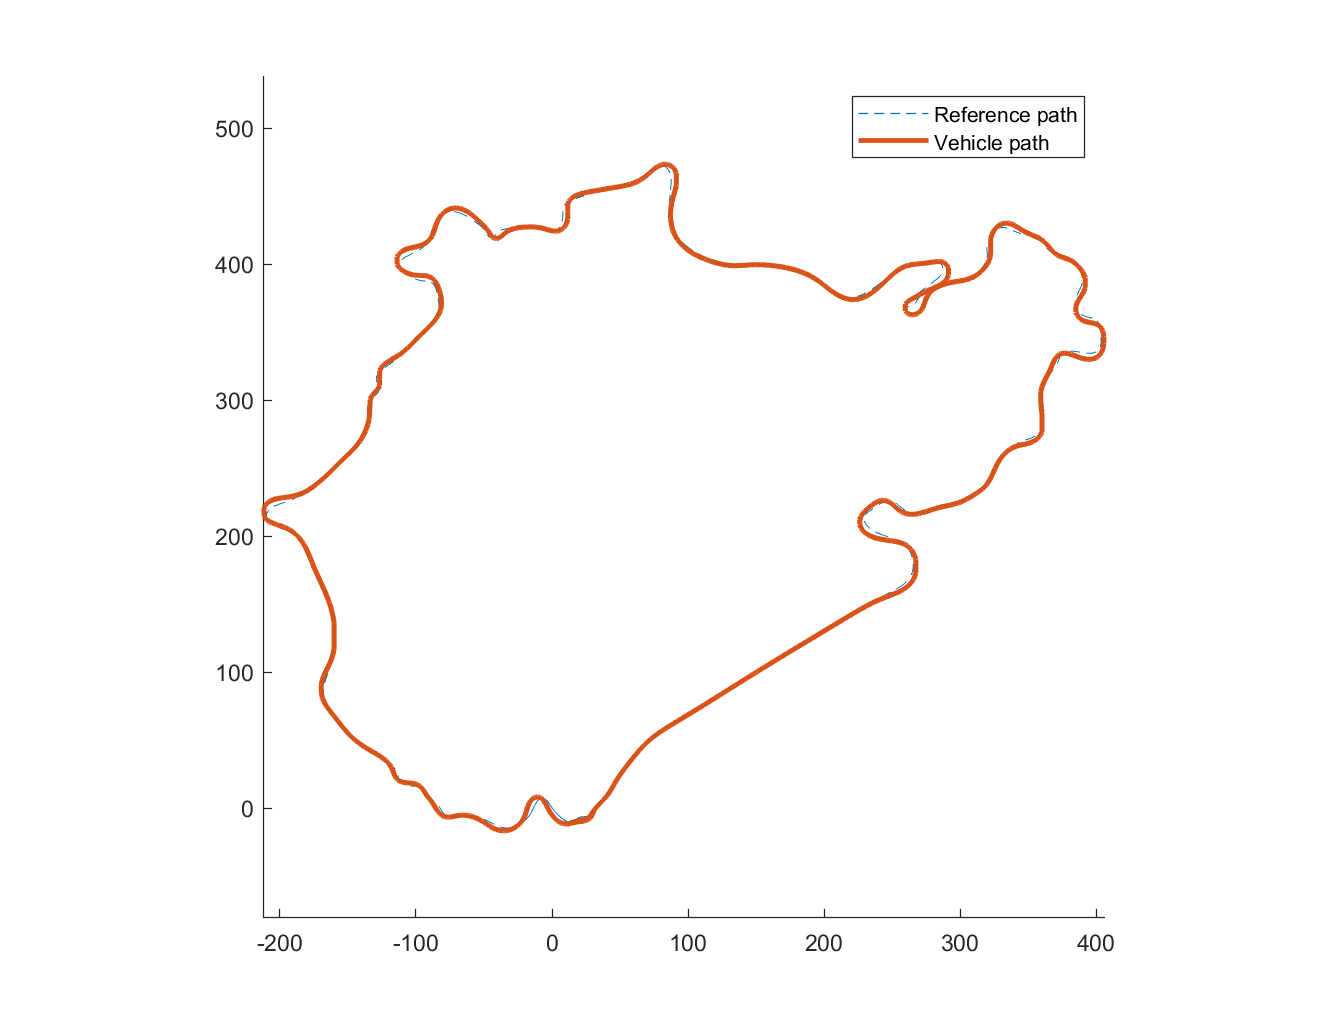
\includegraphics[width=\textwidth]{Latex report/image/ex2/trajectoryNewpole.png}
         \caption{Trajectory}
         \label{fig:NPtraj}
     \end{subfigure}
     \begin{subfigure}[b]{0.8\textwidth}
         \centering
         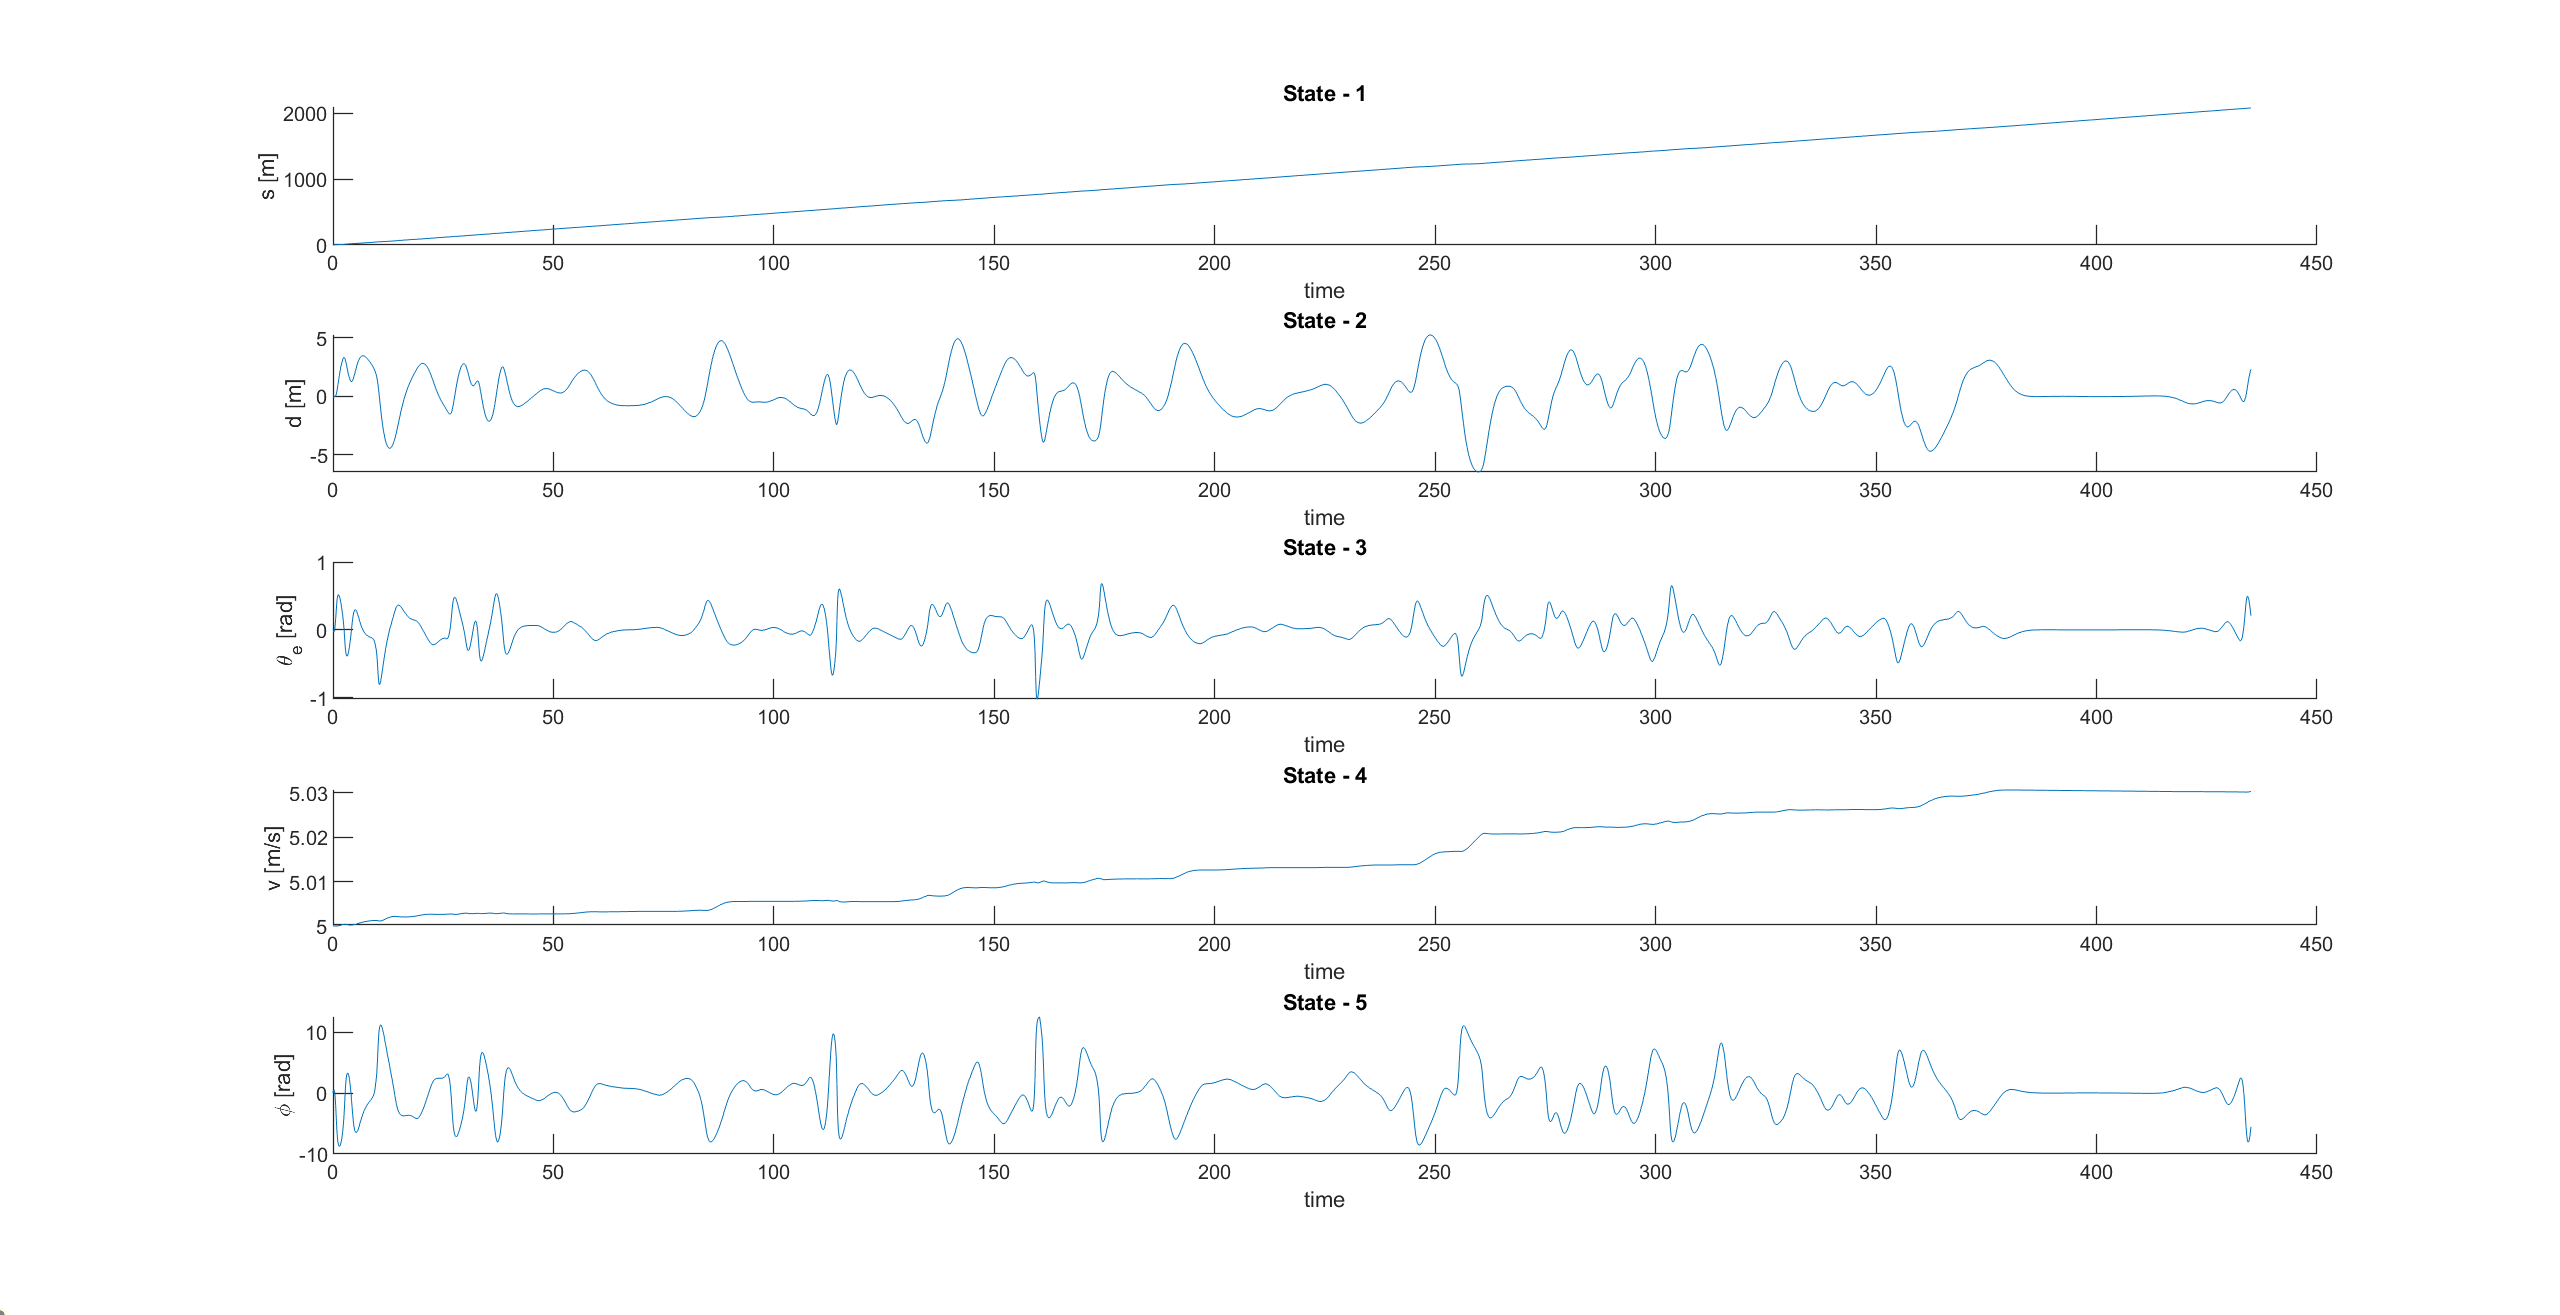
\includegraphics[width=\textwidth]{Latex report/image/ex2/stateNewpole.png}
         \caption{Observed state}
         \label{fig:NPState}
     \end{subfigure}
     \begin{subfigure}[b]{0.8\textwidth}
         \centering
         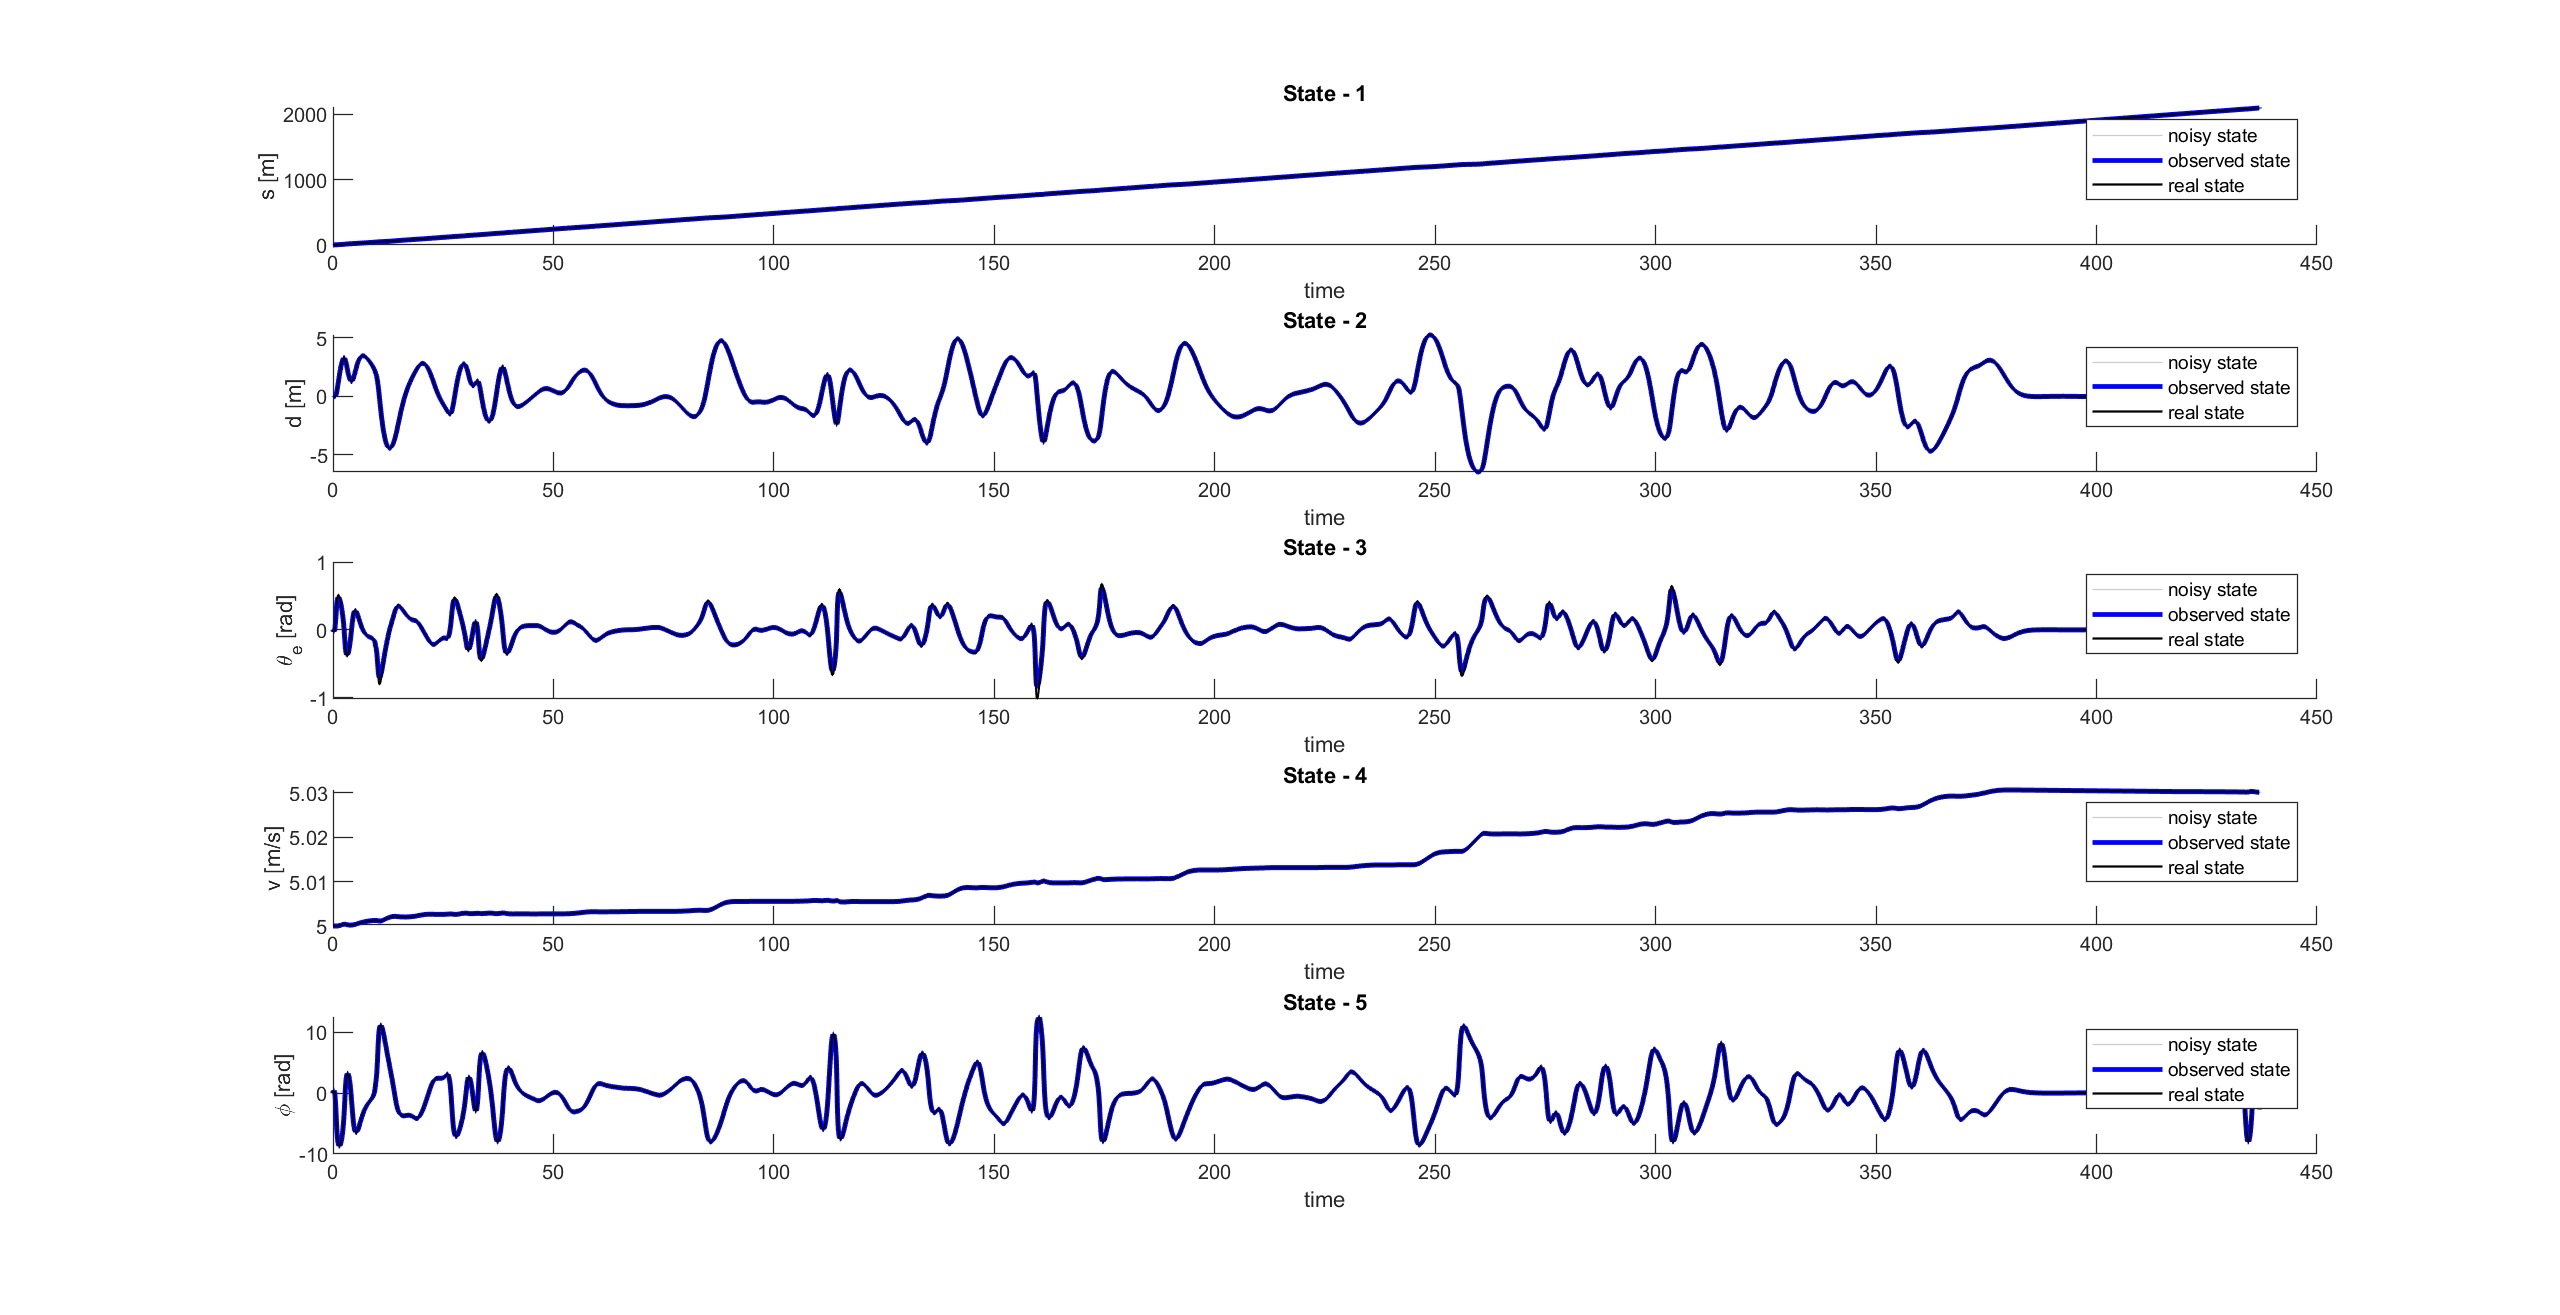
\includegraphics[width=\textwidth]{Latex report/image/ex2/obsNewpole.png}
         \caption{Comparison with state measurement}
         \label{fig:NPObs}
     \end{subfigure}
    \caption{Simulation of the LQR regulator with an observer and new pole placement}
    \label{fig:NP}
\end{figure}

